\chapter{Mathematical Representations of Uncertainty}\label{chap:representation_of_uncertainty}

\section{Introduction}
This chapter takes some distance from the stereo vision problem presented previously, and instead describe more formally different representations of uncertainty and the tools that can be used to manipulate them. In this thesis, we consider classical probabilities (section \ref{sec:probabilities}), possibility distributions (section \ref{sec:possibilities}) and p-boxes (secction \ref{sec:pboxes}) to model uncertainty. We also consider the case where we consider multiple sources of uncertainty simultaneously. In this setting, the dependency between the different sources must be taken into account. We thus present a dependency model called copulas in section \ref{sec:copulas}, and some of its properties. The thorough presentation of those concepts will then be put into relations in chapter \ref{chap:joining_credal_sets}. 

\section{Notations}
We introduce here a few notations that will be used in the rest of this chapter. \todoroman{A ajouter au fur et à mesure, peut être déplacer au début de la thèse, à côté du glossaire.}
\begin{itemize}
    \item \st means ``such that''
    \item We will often present theorems or results with $n$ different variables, spaces, or Cartesian products of $n$ elements. Notations therefore quickly become quite heavy. We try our best to make them clear and readable, which is why we often use the contraction ``$\dots$'' to imply that we are enumerating all variables. For instance, if we apply a function $f$ to four variables $x_1, x_2, x_3, x_4$, we will write $f(x_1, \dots, x_4)$.
    \item When working with $n$ variables, the index $i$ will usually be used to refer to the $i$-th variable (or one of its attribute), and will be appended as a subscript when possible, otherwise as a superscript. For instance, if $x\in\mathbb{R}^n$, then $x_i$ will refer to the $i$-th component of $x$. If $m_\times\in\mathbb{R}^n$, then $m_\times^i$ will refer to $i$-th component of $m_\times$.
    \item $\opi\cdot,\cdot\cli$ refers to an interval of integers. For instance $\opi1,~4\cli=\{1,~2,~3,~4\}$. 
    \item CDF will refer to Cumulative Distribution Function\commanue{Tu n'as pas une section acronymes?}, \ie if $X$ is random variable in $\mathbb{R}$ and $P$ its associated probability, then the CDF of $X$ is $F(x)=P(X\leqslant x)$.
    \item The power set of a set $\X$ is noted $2^\X$. It corresponds to the set of all sets included in $\X$. In the discrete case, if the cardinal of $\X$ is $n$, then the cardinal of the power set is $2^n$, thus the notation.
\end{itemize}

\section{Different Models to Represent Uncertainty}\label{sec:different_models_of_uncertainty}
Assessing the reliability of an engineering system requires to quantify the uncertainty of the input parameters or of the system itself, using models of uncertainty. Modelling the uncertainty can be done in various ways, depending on the type of uncertainty considered and the available measures or \textit{a priori} regarding the uncertain sources. Most common models are probability distributions, which have been studied extensively. When using those models, we know -or suppose- that the information we try to estimate is of stochastic (or random) nature, and that we are able to precisely describe its structure using a probability distribution. However, there are many cases where such assumptions cannot be made: for instance when data is insufficient to determine the correct probability distribution, or when the uncertainty is not random but epistemic. In those cases, we can use other models such as\commanue{Ce serait top de prendre le même exemple et de montrer comment l'incertitude est modélisé différemment, si c'est possible}:
\begin{itemize}
    \item fuzzy sets \cite{zadeh_fuzzy_1999} when trying to estimate the degree of truth of a statement such as ``This person is tall''
    \item intervals \cite{jaulin_applied_2001}, where no preferences are given inside a specific range of possible values
    \item imprecise probabilities which tries to extend the concept of probabilities in order to model epistemic uncertainty
\end{itemize}
This list is not exhaustive. Additionally, those different models can sometimes be equivalent. Choosing to use one or another depends on the nature of the problem and of the available data. In this chapter, we will mainly consider probability distributions (section \ref{sec:probabilities}) and imprecise probabilities (section \ref{sec:imprecise_probabilities}). Two specific cases of imprecise probabilities will be detailed, namely possibility distributions in section \ref{sec:possibilities} and p-boxes in section \ref{sec:pboxes}.

At the end of the day, choosing one model over another is not always straightforward. It requires to be aware of the type of uncertainty faced, of the strengths and limitations of each model, of the tools available to manipulate the models \etc When it comes to less common models cited above, it fundamentally requires to be aware of the existence of such models, which is not always the case for non-specialists. During this thesis, we tried to promote less common models, especially possibility distributions. We did so by presenting real life cases where they could be used while improving uncertainty modeling in the field of stereo-photogrammetry (see chapters \ref{chap:propagating} and \ref{chap:epistemic_uncertainty}). \comroman{Je pense que cette remarque devrait plutôt se retrouver dans l'intro de la thèse, car elle s'éloigne de ce qui suit. Peut être même que les deux paragraphes pourraient être déplacés dans l'intro}\commanue{Oui tu peux mettre cela dans l'intro, ce sera mieux. Après la remarque est très bien}

\subsection{Probabilities}\label{sec:probabilities}
Probability measures are a classical framework to represent uncertainty. There are multiple ways of interpreting them, mainly with a \textit{frequentist} approach, or a \textit{Bayesian} approach. From a frequentist point of view, probabilities are well fitted to represent stochastic uncertainty, \ie uncertainty regarding events that can get a different result each time we run an experiment or acquire a measure (typically, noise on a sensor). From a \textit{Bayesian} point of view, probabilities represent a state of knowledge or degree of belief, and can be updated with additional information. This leads to the notion of prior and posterior probability that will not be considered in this thesis.

We remind here basic definitions regarding probability distributions.
\begin{definition}[Probability Space]\label{def:probability_space}
    We call a probability space $(\X,~\mathcal{A},~P)$ a tuple where:
    \begin{itemize}
        \item $\X$ is the set of possible outcomes (for instance head or tails for a toss coin), also called frame of discernment.
        \item $\mathcal{A}$ is the set of all subsets of $\X$ for which a probability can be measured (for instance $\{\emptyset, \{\text{heads}\}, \{\text{tails}\}, \{\text{heads, tails}\}\}$)
        \item $P$ is the probability measure assigning a probability to each of the sets of $\mathcal{A}$. For instance for a fair coin, $P(\emptyset)=0$, $P(\{\text{heads}\})=P(\{\text{tails}\}=0.5$ and $P(\X)=1$.
    \end{itemize}
    Note that $\mathcal{A}$ must be a $\sigma$-algebra meaning that it is closed under complement, countable unions and countable intersections. $P$ is a probability measure if it verifies all the Kolmogorov axioms:
    \begin{itemize}
        \item $\forall A\in\mathcal{A},~P(A)\in[0,1]$
        \item $P(\X) = 1$
        \item for any countable disjoint family of sets $A_i\in\mathcal{A}$, $P(\cup_i A_i)=\sum_i~P(A_i)$
    \end{itemize}
\end{definition}

\begin{definition}[Random Variable]
    A random variable $X$ is a measurable function from $\X$ to a measurable space (which is often $\mathbb{R}$ or a subset of $\mathbb{R}$). We can then measure the probability that $X$ takes a value in $E\subseteq\mathbb{R}$\commanue{Pourquoi E est inclus dans R. Ton sous-ensemble E ne devrait pas inclus dans un espace mesurable noté la lettre que tu veux}:
    \begin{align*}
        P(E) = P(\{x\in\X~|~X(x)\in E\})
    \end{align*}
\end{definition}

Using a random variable allows to consider the probability measure on different spaces. We then call $P$ the probability distribution of the considered random variable $X$.

Other useful concepts regarding probability distributions are cumulative distribution functions and density functions:
\begin{definition}[Cumulative Distribution Function]\label{def:cdf}
    A Cumulative Distribution Function $F_X$ of a random variable $X$ with real values is the probability that $X$ will be less or equal to a number $x$. Formally, we define $F_X:\X\rightarrow[0,1]$:
    \begin{equation*}
        \forall x\in\X,~F_X(x)=P(X\leqslant x)
    \end{equation*}
\end{definition}

\begin{definition}[Density Function]\label{def:density}
    A random variable $X$ is said to possess a density function if there exists a positive integrable function $f$ over $\mathbb{R}$ \st $\forall (x_1, x_2)\in\mathbb{R}^2$:
    \begin{equation*}
        P(x_1\leqslant X \leqslant x_2) = \int_{x_1}^{x_2}f(x)dx
    \end{equation*}
    In the discrete case, the density is also called \textit{probability mass function}, and is defined as \commanue{Alors wikipedia me donne un signe $=$ et pas $\leqslant$ mais je regarde peut-être pas le bon truc}:
    \begin{equation*}
        f(x_1) = P(X \leqslant x_1)
    \end{equation*}
    In the continuous case, the density $f$ is also the derivative of the CDF of $X$\commanue{Je mettrais la remarque avant la partie discrète}.
\end{definition}
%For instance, the uniform distribution on the interval $[1,100]$ has a density function $f(x)=\frac{1}{100-1}$ if $x\in[1,100]$ and $0$ elsewhere. Its CDF is thus $0$ if $x<1$, $\frac{x}{100-1}$ if $x\in[1,100]$ and $1$ elsewhere. The concept of a CDF for multiple variables will be explored in section \ref{sec:copulas}.

In the rest of the chapter, we consider random variables $X$ on discrete spaces $\X$. If $\X=\{x_1,~\dots,~x_n\}$, we call $\{x_i\}$ an atom of $\X$, and the probability distribution $P$ of $X$ on $\X$ is completely determined by its density, which is the value of $P$ on atoms. For simplicity of notation, we will not always use braces around atoms when computing their probability. So we will sometimes write $P(x_1)$ instead of $P(X=\{x_1\})$.

As stated previously, probability measures are fitted to represent stochastic uncertainty. The following example illustrates why probability measures are not adapted to represent epistemic uncertainty:
%%%% Complex example, a simpler one is presented bellow
%\begin{example}
%    Consider a thermometer measuring the temperature of an unknown container. We only know that the temperature is above $1$ and bellow $100$ degrees Celsius. We define $X:\X\rightarrow[1,~100]$ as the random variable representing the output of the thermometer and are interested in its value. In the absence of further information on the container, a common procedure is to associate the uniform distribution to $X$. The CDF $F_X$ of $X$ is thus:
%    \begin{equation*}
%        \forall x\in\mathbb{R},~CDF_X(x)=\mathds{1}_{[1,~100]}(x)\frac{x}{100-1}
%    \end{equation*}
%    We now consider a random variable $Y$ defined as the logarithm of $X$: $Y=\ln X$. We still do not have any further information on the device and we have thus no preference on the values of its logarithm. Following the method above, one could also be tempted to associate a uniform distribution to $Y$. However, computing the CDF $F_Y$ of $Y$ from that of $X$ yields for all $y$:
%    \begin{align*}
%        F_Y(y) &= P(Y\leqslant y) = P(\ln(X)\leqslant y) = P(X \leqslant e^y) = F_X(e^y)\\
%        &= \mathds{1}_{[1,~100]}(e^y)\frac{e^y}{100-1}
%    \end{align*}
%    Which is clearly not the CDF of a uniform distribution. This is because a uniform distribution is well suited for representing statements like ``all values have the same likelyhood'' but not for statements like ``I have no information over the values (and thus no preference)''. In general, probability distributions cannot represent epistemic uncertainty as a probability distribution actually contains a lot of information about a random variable.    
%\end{example}
\begin{example}\label{ex:proba_limitations}
    Let consider a card facing down, with a number written on its hidden side. The person who wrote the number tells you that they chose to wrote either $1$, $2$ or $3$ on it. We should not that because they chose to write a number, the uncertainty on its value is not random. They then ask you to evaluate your chances of guessing the correct number and its parity, \ie if it is odd or even. We first consider the random variable $X$ taking values in $\{1,~2,~3\}$. Because you have no further information and thus no preferences on the values of $X$, a common (yet false) decision is to associate the uniform distribution $P$ to $X$:
    \begin{equation*}
        P(X=1)=P(X=2)=P(X=3)=\frac{1}{3}
    \end{equation*}
    For the parity of the number, we may now consider the random variable $Y$ defined such that $Y=0$ if ``$X=1$ or $X=3$'' and $Y=1$ if ``$X=2$''. Because we have no information on the number written on the card, we also do not have any preferences on the values of $Y$. Following the same reasoning as before, one might be tempted to associate an uniform distribution to it. However, deducing the density of $Y$ from that of $X$ yields:
    \begin{equation*}
        P(Y=0)=P(X=1)+P(X=3)=\frac{2}{3},\qquad P(Y=1)=P(X=2) = \frac{1}{3}
    \end{equation*}
    Which is clearly not the density of an uniform distribution. By supposing we have no preferences on the values of a variable, we actually deduced preferences on the values of another variable. One should use an uniform distribution only when they are certain that all values are equiprobable. This is because uniform distributions are well suited for representing statements like ``all values have the same likelyhood'' but not for statements like ``I have no information over the values, and thus no preference''. Indeed, a probability distribution actually contains a lot of information about a random variable, which is not suited to represent epistemic uncertainty.\commanue{J'aime bien l'exemple il faudrait peut-être juste ajouter des mots de liaison pour bien distinguer les différents raisonnements entre eux.}
    
    \begin{remark}
        From a Bayesian point of view, a probability can also represent a degree of belief, allowing them to represent epistemic uncertainty and not only stochastic uncertainty, in theory. However, it does not solve the expressiveness problem raised by this example. Bayesians are still reasoning with probabilities, which make no difference between ``I have no preference between these events'' and ``these events are equiprobable''. Even though they can update their prior with additional information, this would not fix the problem presented here. In the absence of additional information, basing a decision on the prior would lead to debatable conclusions.
    \end{remark}
\end{example}

\subsection{Imprecise Probabilities}\label{sec:imprecise_probabilities}
As highlighted in example \ref{ex:proba_limitations}, uncertainty cannot always be correctly modeled by probabilities, especially in a context where data is sparse. To overcome this problem, a generalization of probabilities have been introduced, called \textit{imprecise probabilities}. Imprecise probabilities (sometimes abbreviated IP) provide a general framework for working with both aleatoric and epistemic uncertainty with the concept of lower and upper probabilities. Lower and upper probabilities are quite  generic and flexible, and can be derived in more specific models. Here is a brief scope of the relevant tools it compasses: the special case of \textit{belief functions}, themselves containing specific sub-categories such as possibility distributions \ref{sec:possibilities} and probability boxes \ref{sec:pboxes} \etc\commanue{Je mettrais pas le etc} It also contains probabilities presented in section \ref{sec:probabilities}, which we will call \textit{precise} probabilities by opposition to \textit{imprecise} probabilities. Figure \ref{fig:diagram_IP} sums up the relationship and specificity of each imprecise model.

\begin{remark}
    At its more generic, IP can be described by sets of acceptable gambles, and by lower and upper expectations \cite{walley_statistical_1991,augustin_introduction_2014}. Although very interesting, we did not use them in our applications and thus do not consider them in this thesis.
\end{remark}
\begin{figure}[ht]
    {\centering
    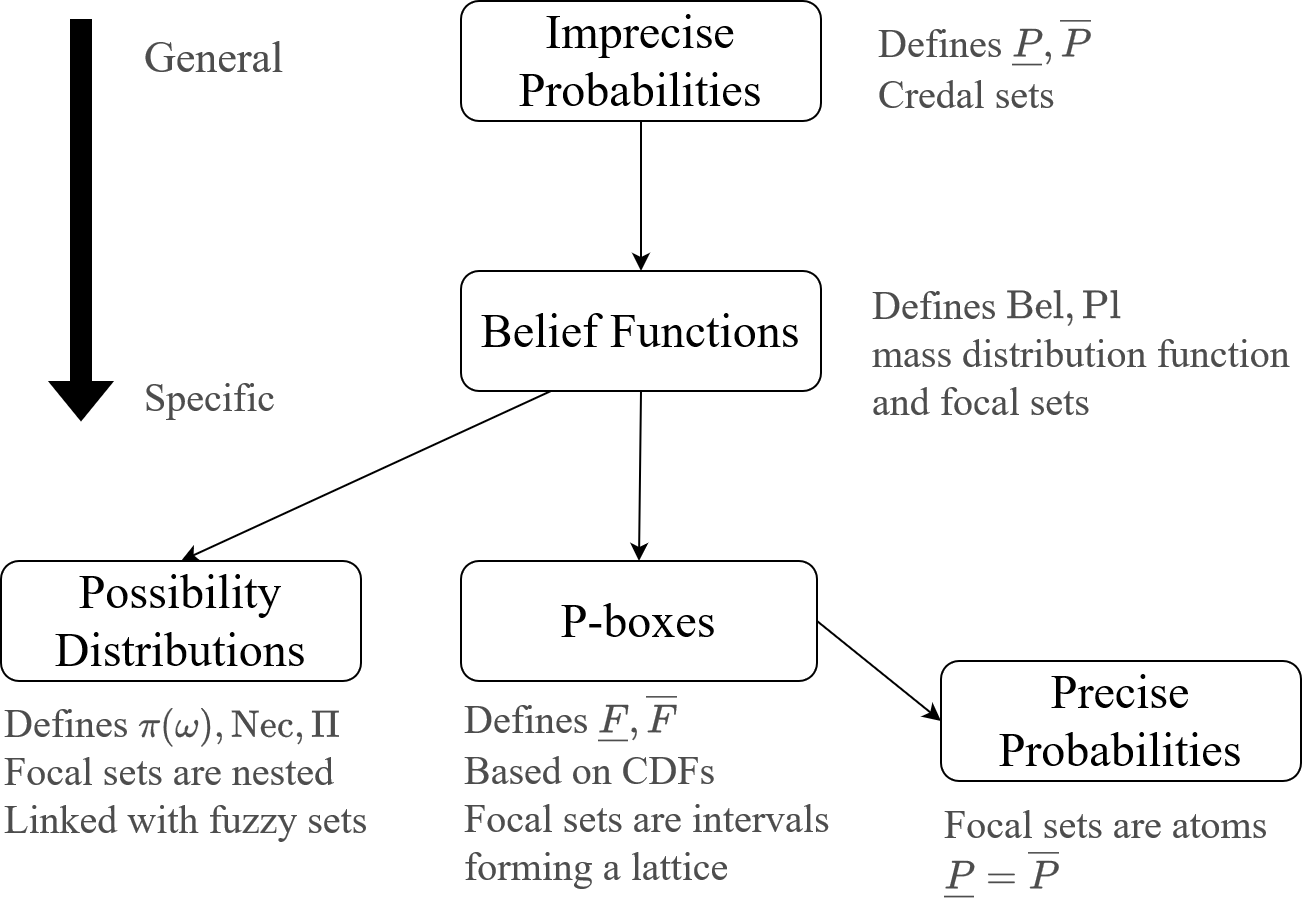
\includegraphics[width=0.8\linewidth]{Images/Chap_2/Diagramme_IP_Bel.png}
    \caption{Diagram representing the relationship between different Imprecise Probabilities models presented throughout section \ref{sec:different_models_of_uncertainty}.}
    \label{fig:diagram_IP}}
\end{figure}\commanue{La figure est bien pour voir les liens après je ne sais pas s'il faut garder les éléments en gris clair, c'est un peu déroutant pour le lecteur qui découvre les éléments}

As stated previously, a core concept of imprecise probabilities are lower and upper probabilities. Similarly to precise probabilities, a lower probability $\low$ and an upper probability $\overline{P}$ are mappings from a $\sigma$-algebra $\mathcal{A}$ to $[0, 1]$. However, while a probability $P$ gives a single measure of uncertainty for every event, lower and upper probabilities provide two bounds for every event, allowing them to express more complex uncertainty structures.

\begin{remark}
    Formally, a lower probability $\low$ needs to be \textit{super-additive}, \ie to verify:
    \begin{equation}
        \forall A,B\in\mathcal{A}, \text{ if } A\cap B\neq\emptyset, ~\low(A\cup B)\geqslant \low(A)+\low(B) \label{eq:super_additivity}
    \end{equation}
    Conversely, an upper probability is sub-additive, meaning that it verifies the same property than equation \eqref{eq:super_additivity} but with the inequality reversed.
    
    Those properties are less constraining than their equivalent for precise probabilities in definition \ref{def:probability_space}, so lower and upper probabilities are generally \textit{not} precise probabilities. The only case where they are precise probabilities is when $\low=\overline{P}$, because $\low$ is then additive as it is both super and sub-additive. In this case, imprecise probabilities are actually a single precise probability. This illustrates the fact that precise probabilities are special cases of imprecise probabilities. 
\end{remark}

Precise probabilities define a measure of uncertainty towards a random variable $X$ taking numerical values. Imprecise probabilities however, can model the uncertainty towards a random variable taking set values instead of numerical one. We then say that $X$ is a \textit{random set} instead of a random variable. That being said, IP can also represent the uncertainty of random variables for which we suppose a precise probability exists, but we are not able to determine it precisely. Indeed, lower and upper probabilities form the bounds of a family of precise probabilities called \textit{credal set}.
\begin{definition}[Credal set]\label{def:credal_set}
    Given a lower probability $\low$ and an upper probability $\overline{P}$, a credal set $\M$ is the set of all probabilities $P$ that are greater that $\low$ and lower that $\overline{P}$:
    \begin{equation}
        \M(\low, \overline{P}) = \{P~|~\forall A\in\mathcal{A},~\low(A)~\leqslant~P(A)~\leqslant\overline{P}(A)\}
    \end{equation}
\end{definition}
We refer to $\M(\low, \overline{P})$ as $\M$ when no confusion is possible. Credal sets allow to consider multiple probabilities at once, which improves on the limited expressiveness of a single probability measure. The gap between the two bounds of a credal set reflects how imprecise is the model, in terms of epistemic uncertainty.

Conversely, we can define lower and upper bounds from a set of probabilities $\M$ as:
\begin{align*}
    \forall A\in\mathcal{A},~\low(A) =& \inf_{P\in\M}P(A)\\
    \forall A\in\mathcal{A},~\overline{P}(A) =& \sup_{P\in\M}P(A)
\end{align*}

Although, it is not required, we usually assume credal sets verify additional properties expressed as follows:
\begin{definition}[Coherence and Avoiding sure loss]\label{def:coherence_sure_loss}
    A credal set $\M$ is said to avoid sure loss if it contains at least one probability measure, \ie if
    \begin{equation}
        \M \neq \emptyset\label{eq:avoid_sure_loss}
    \end{equation}
    
    A credal set $\M$ is said to be \textit{coherent} if its lower bounds an all events are attained by a probability measure, \ie if \commanue{C'est pas low(A) = P(A) dans l'équation et la phrase ne mentione upper bounds, j'ai l'impression qu'il te manque un bout ou c'est mon anglais qui est nul}:
    \begin{equation}
        \forall A\in\mathcal{A}, \exists P, P'\in\M~\st~\low(A)=A \text{ and } \overline{P}(A)=P'(A) 
    \end{equation}
\end{definition}
The bounds $\low, \overline{P}$ of a coherent credal set verifies the following property:
\begin{equation}
    \forall A\in\mathcal{A}, ~\low(A) = 1 - \overline{P}(A^c)\label{eq:lower_proba_complement}
\end{equation}
which is a generalization of the classical property for computing the complement of an event with precise probabilities. This allows us to only specify the lower bound $\low$ of a credal set to completely describe it, as its upper bound is determined by $\low$. Defining a credal set requires to specify much more constraints on the probability space that in the case of probability distributions. Indeed a lower probability must be defined on every possible event, while a precise probability can be defined by its density on possible values only (instead of possible events). In the case of a discrete space with $n$ elements, a probability is completely determined by its values on the $n$ atoms, while a lower bound is completely determined by its values on the $2^n$ considered events.


\begin{remark}
    Sampling from a credal set is not straightforward. Multiple method exists, the most intuitive consisting in sampling distributions from the credal set extreme points.
\end{remark}

\begin{remark}
    With the way we defined a credal set $\M$, it is closed and convex. This is a common way of constructing credal sets, but is not the only way. We could for instance impose that all probabilities in $\M$ belong to a family of Gaussian probabilities, which would prevent $\M$ from being convex.
\end{remark}

When constructing credal sets, it is common to possess a non convex set of probabilities $S$. In that case, we can define the convex hull of a set of probabilities $S$:
\begin{definition}[Convex Hull]\label{def:convex_hull}
    The convex hull ($CH$) of a set of probabilities $S$ is the smallest (convex) credal set containing $S$:
    \begin{equation}
        CH(S) = \{~P~|~\forall A\in\mathcal{A}, ~\inf_{P_S\in S}P_S(A)\leqslant P(A) \leqslant \sup_{P_S\in S}P_S(A)\}
    \end{equation}
\end{definition}

\begin{remark}
    The convex hull is computationally heavy to compute. Determining the infimum and supremum of a set of probability is not trivial as it might require to iterate through every element of $S$. It is however very useful, especially in the case where we do not know the set bounds on every event. In that case, computing the convex hull also allows us to determine the bounds on those events.
\end{remark}

\begin{example}
    Let us consider the scenario presented in example \ref{ex:proba_limitations}, and model the uncertainty with a credal set instead of a single probability distribution. Because we have no information on the value written on the card except that it is in $\{1,2,3\}$, we characterize the uncertainty by lower and upper probability $\low$, $\overline{P}$ defined as follows:
    \begin{align*}
        &\low(X=1) = \low(X=2)= \low(X=3) = 0\\
        &\overline{P}(X=1) = \overline{P}(X=2)= \overline{P}(X=3) = 1\\
        &\low(X\in\{1,2,3\}) = \overline{P}(X\in\{1,2,3\}) = 1
    \end{align*}
    We can use equation \eqref{eq:lower_proba_complement} for computing the bounds of remaining events.
    
    Here, the credal set is the largest credal set possible as its bounds are always $0$ and $1$ for events that are not $\emptyset$ or $\{1,2,3\}$. We say that it is the vacuous credal set, as it does not encode any information. It however solves the problem of a contradicting probability when evaluating the value of the card and its parity.\commanue{J'aime bien le fait de présneter l'exemple. Après j'ai des difficultés à comprendre les deux dernières phrases.}
\end{example}

\subsection{Belief Functions}\label{sec:belief_functions}
A special case of imprecise probabilities are belief functions, which we will detail in this section. First, we will introduce a key concept that goes along belief functions: mass distribution functions. We will then derive belief functions from it.

\begin{definition}[Mass distribution function]\label{def:mass_distribution_function}
    Let $\X$ be a frame of discernment\commanue{alrs X à la base c'est set of possible outcomes et là tu donnes un autre nom c'est pour la même chose ou il y a une subtilité. J'aime pas les variables qui changent surtout quand je suis pas à l'aise dans le domaine} and $2^\X$ its power set. A mass distribution function (or basic probability assignment \cite{shafer_mathematical_1976}) is a function $m:2^\X\rightarrow[0,1]$ \st:
    \begin{align}
        m(\emptyset) =& 0\label{eq:mass_emptyset}\\
        \sum_{a\subseteq\X}m(a) =& 1\label{eq:mass_whole_set}
    \end{align}
\end{definition}

There are multiple ways of interpreting $m(a)$, presented bellow so as to be more familiar with $m$:
\begin{itemize}
    \item If we consider a random set $X$, then $m(a)$ encodes the probability mass that $X$ takes $a$ as its set value.
    \item If $X$ is a random variable, then $m(a)$ encodes the available evidence that the numerical value of $X$ is \textit{exactly} in $a$, without any preferences for the values within $a$. This mean there could also be another evidence that $X$ is in $a'\subset a$, encoded with $m(a')$, and which could be either lower or higher than $m(a)$ depending on the amount of evidence available. Example \ref{ex:bicycle_pressure} illustrates this with a toy scenario. 
    \item Another interpretation of $m(a)$ is to link it to probability masses (definition \ref{def:density})\commanue{C'est bizarre de dire anaother car le premier parle déjà du lien entre m(a) et probability mass. Peut-être dire precise probability mass pour que ce soit plus clair}. If we suppose there exists an unknown underlying probability measure $P$ for $X$, $m(a)$ measures the probability mass that is assigned to $a$, but that can move freely to every point of $a$ without any preference. In other words, with more information, we could distribute $m(a)$ to every elements of $a$, and doing this for all $a$ would lead to a precise probability mass distribution.
\end{itemize}

\begin{remark}
    Equation \eqref{eq:mass_emptyset} translates the fact than there is no evidence that the uncertain variable belongs to the empty set, \ie that it is not defined. Releasing this constraint allows to accept a certain amount of contradiction in our model.
    Equation \eqref{eq:mass_whole_set} is a convention, which states that the total amount of evidence equals $1$. It is similar to probabilities which cannot be more than $1$. 
\end{remark}

\begin{definition}[Focal set]\label{def:focal_set}
    Let $\X$ be a frame of discernment\commanue{Même remarque que précédemment sur X}, $2^\X$ its power set, and $m:2^\X\rightarrow[0,1]$ a mass distribution function. A set $a\subseteq\X$ is called a focal set of $m$ if and only if:
    \begin{align}
        m(a)>0\label{eq:focal_set}
    \end{align}
\end{definition}
Focal sets thus represent sets of the frame of discernment for which we have evidence. The set of all focal sets is sometimes called the \textit{core} of $m$.

\begin{definition}[Belief function, Plausibility function]\label{def:belief_plausibility}
    Let $\X$ be a frame of discernment, $2^\X$ its power set, and $m:2^\X\rightarrow[0,1]$ a mass distribution function.
    
    We define the belief function associated with $m$ as the function $\Bel:2^\X\rightarrow[0,1]$ who associates to all events $A$ in $2^\X$:
    \begin{align*}
        \Bel(A)=\sum_{a\subseteq A} m(a)
    \end{align*}
    
    We define the plausibility function associated with $m$ as the function $\Pl :2^\X\rightarrow[0,1]$ who associates to all events $A$ in $2^\X$:
    \begin{align*}
        \Pl(A)=\sum_{\substack{a\\a\cap A\neq\emptyset}} m(a)
    \end{align*}
\end{definition}
We can interpret $\Bel(A)$ as the amount of evidence that fully support $A$, and $\Pl(A)$ as the amount of evidence that is consistent (or does not contradict) with $A$.

$\Bel$ and $\Pl$ are special cases of lower and upper probabilities, and verify \eqref{eq:lower_proba_complement} as for all events $A$ it holds:
\begin{align*}
    \Bel(A)&=\sum_{a\subseteq A} m(a)\\
    &= \sum_{a\in \X} m(a) - \sum_{a\not\subseteq A} m(a)\\
    &= 1 - \sum_{\substack{a\\a\cap A^c\neq\emptyset}} m(a)\\
    &=1-\Pl(A^c)
\end{align*}

Belief functions possess interesting properties making the credal set they induce both coherent and avoiding sure loss, motivating their extensive usage.

\begin{example}[Defining mass and belief\commanue{manque plausibility} functions]\label{ex:bicycle_pressure}
    Let us imagine an experiment where you try to estimate the pressure of the tyres of your bike, but your bicycle pump only have graduation every $1$ bar. You are able to do three measurements:
    \begin{itemize}
        \item The first measure, the needle seems to be between $4$ and $5$ bar.
        \item The second measure, the needle seems to be between $4.5$ and $6$ bar.
        \item The third measure, the needle seems to be between $4.5$ and $5.5$ bar.
    \end{itemize}
    Let us say that you trust your last measurement the most, because you got used to the movement of the needle. It is now possible to model the uncertainty of your tyre pressure using available evidence encoded in $m$:\\
    \noindent
    \begin{minipage}{0.3\textwidth}
        \begin{align*}
            m([4,~5]) ~=~ 0.3
        \end{align*}
    \end{minipage}\hfill
    \begin{minipage}{0.3\textwidth}
        \begin{align*}
            m([4.5,~6]) ~=~ 0.3
        \end{align*}
    \end{minipage}\hfill
    \begin{minipage}{0.3\textwidth}
        \begin{align*}
             m([4.5,5.5]) ~=~ 0.4
        \end{align*}
    \end{minipage}\par
    Based on this, we are no able to express our degree of belief and of plausibility for all events. For instance:
    \begin{itemize}
        \item Our degree of belief that the pressure lies in $[4, 5]$ is $\Bel([4, 5])=0.3$, that it lies in $[4, 5.5]$ is $\Bel([4, 5.5])=0.7$ and that it lies in $[4, 6]$ is $\Bel([4, 6])=1$
        \item The degree of plausibility that the pressure equals $5$ is $\Pl (5)=1$ (totally plausible), that it equals $5.5$ is $\Pl (5.5)=0.7$ and that it equals $4$ is $\Pl (4)=0.3$.
    \end{itemize}
\end{example}

\subsection{Possibility Distributions}\label{sec:possibilities}
Another convenient model of uncertainty are possibility distributions. We will see that they induce a particular type of belief functions, and will be used in our applications.

\begin{definition}[Possibility distribution]\label{def:possibility}
    Let $\X$ be the frame of discernment. A possibility distribution is a function $\pi: \X \rightarrow [0,1]$ satisfying:
    \begin{equation}
    	\exists x \in \X, \pi(x) = 1 \label{eq:possibility}
    \end{equation}
    The value $\pi(x)$ represents the degree of possibility of $x$, with $\pi(x) = 1$ indicating full possibility, and $\pi(x) = 0$ indicating impossibility.
\end{definition}

Another notion closely related to possibility distributions is that of \(\alpha\)-cuts:
\begin{definition}[\(\alpha\)-cut]\label{def:alpha_cut}
    Let $\pi: \X \rightarrow [0,1]$ be a possibility distribution. Given any \(\alpha\in[0,1]\), we define the \(\alpha\)-cut of \(\pi\) as:
    \begin{align}
        \alpha_\pi=\{x~|~\pi(x)\geqslant\alpha\} \label{eq:alpha_cut}   
    \end{align}
    An \(\alpha\)-cut is thus the set of all elements of $\X$ whose possibility level is more that $\alpha$.
\end{definition}

\begin{definition}[Necessity and Plausibility\commanue{c'est pas possibility? Plausibility c'est déjà défini au-dessus}]
    It has been proven in \cite{dubois_when_1992} that a possibility distribution defines a specific type of plausibility functions called \textit{possibility} function and noted \(\Pi\). It also defines a specific belief function by duality called \textit{necessity} function and noted \(\Nec\), as well as a credal set $\M(\pi)$. They are defined as\commanue{Tu veux pas direct mettre possiblity et necessity dans la définition du credal set}:
    \begin{align}
        &\Pi(A) = \sup_{x\in A}\pi(x)\\
        &\Nec(A)=1-\sup_{x\in A^c}\pi(x)\label{eq:bel_pl}\\
        &\M(\pi)=\{P~|~\forall A,~P(A)\leqslant \sup_{x\in A}\pi(x)\}\label{eq:credal_set_possibility}
    \end{align}
\end{definition}

\begin{example}[Defining a possibility distribution]\label{ex:bicycle_pressure_possibility}
    Let us imagine the same setting as example \ref{ex:bicycle_pressure}, where we try to estimate the pressure of the tyres of our bike, but our bicycle pump only have graduation every $1$ bar. We are able to do the following measurements:
    \begin{itemize}
        \item During the first measurement, the needle seems to be around $4$ bar.
        \item During the second measurement, the needle seems to be around $5$ bar.
        \item During the third measurement, the needle seems to be around $4.5$ bar.
    \end{itemize}
    Let us say that we trust our measurement with a precision of plus or minus $0.5$ bars. For simplicity, we also only consider pressure values that are integers or half integers. Taking into considerations all the measurements, we can define a possibility distribution $\pi$ as:
    \begin{itemize}
        \item The value of $4.5$ being the most possible, $\pi(4.5)=1$.
        \item Values between $4$ and $5$ bar being mostly possible, we can for instance fix $\pi(4)=\pi(5)=0.8$
        \item Values $3.5$ and $5.5$ are unlikely but not impossible, we can say that $\pi(3.5)=\pi(5.5)=0.3$
        \item Other values are impossible, and thus have a possibility of $0$.
    \end{itemize}
    The possibility distribution $\pi$ is represented in figure \ref{fig:possibility_distribution}
    Based on this, we are no able to express the degree of necessity and of possibility for all events. For instance:
    \begin{itemize}
        \item The degree of necessity that the pressure lies between $4$ and $5$ bar is $\Nec([4, 5])=1-\sup_{\rho\not\in[4,5]}\pi(\rho)=0.7$
        \item The degree of necessity that the pressure lies between $3.5$ and $5.5$ bar is $\Nec([3.5,~ 5.5]) = 1-\sup_{\rho\not\in[3.5,5.5]}\pi(\rho) = 1$\comroman{Retour à la ligne avant l'équation?}, meaning that the pressure is necessarily in this range.
        \item The degree of possibility that the pressure is either $3.5$ or  $5$ is $\Pi (\{3.5,~5\})=\sup_{\rho\in\{3.5,~5\}}\pi(\rho)=0.9$ (mostly possible).
        \item \etc for every possible event.
    \end{itemize}
\end{example}

\begin{figure}[!ht]
    \centering
    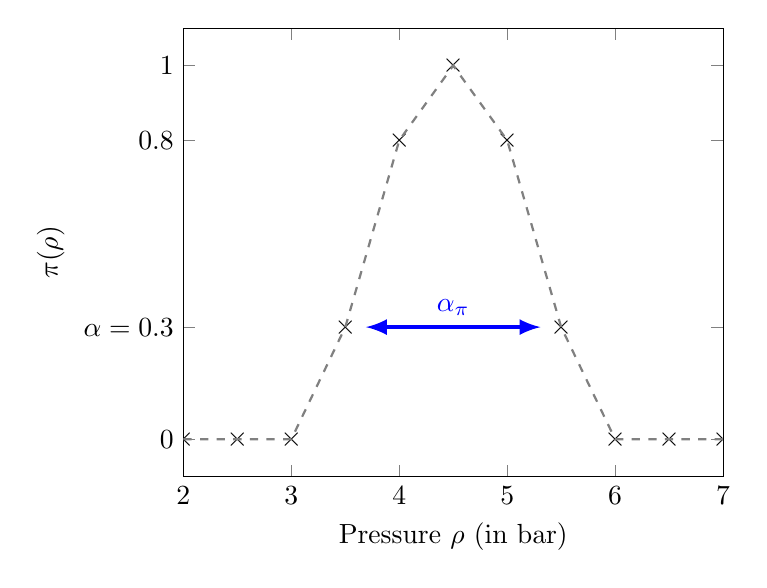
\begin{tikzpicture}[scale=1]
        \begin{axis}[%
          xlabel=Pressure $\rho$ (in bar),
          ylabel=$\pi(\rho)$,
          xmin=2, xmax=7,
          ymin=-0.1, ymax=1.1,
          ytick={0, 0.3, 0.8, 1},
          yticklabels={$0$, $\alpha=0.3$, 0.8, $1$},
          ],
          \node (a) at (2, 0) {$\times$};
          \node (b) at (2.5, 0) {$\times$};
          \node (c) at (3, 0) {$\times$};
          \node (d) at (3.5, 0.3) {$\times$};
          \node (e) at (4, 0.8) {$\times$};
          \node (f) at (4.5, 1) {$\times$};
          \node (g) at (5, 0.8) {$\times$};
          \node (h) at (5.5, 0.3) {$\times$};
          \node (i) at (6, 0) {$\times$};
          \node (j) at (6.5, 0) {$\times$};
          \node (k) at (7, 0) {$\times$};
          
          \draw [thick, dashed, gray] (a.center) -- (b.center) -- (c.center) -- (d.center) -- (e.center) -- (f.center) -- (g.center) -- (h.center) -- (i.center) -- (j.center) -- (k.center) ;
          \draw [<->, >=latex, ultra thick, blue] (d.east) -- (h.west) node [pos=0.5, above] {$\alpha_\pi$};
        \end{axis}
    \end{tikzpicture}
    \caption{Possibility distribution of example \ref{ex:bicycle_pressure_possibility} and one of its $\alpha$-cut in blue}
    \label{fig:possibility_distribution}
\end{figure}

\begin{remark}
    If you are familiar with fuzzy sets you may have noticed than possibility distributions strongly resemble to the membership function of a fuzzy set. Links between fuzzy sets and possibility measures have been explored in \cite{zadeh_fuzzy_1999}.
\end{remark}

Focal sets of necessity functions can be determined directly from the possibility distribution by looking at their \( \alpha \)-cuts. It has been proven that the core $\mathcal{C}$ (the set containing all focal sets) of a necessity function is (\cite{destercke_unifying_2008}):
\begin{align*}
    \mathcal{C} =& \{\alpha_\pi~|~\alpha\in[0,1]\}\\
    =& \{ ~\{x\in\X~|~\pi(x)\geqslant\alpha\}~|~\alpha\in[0,1]~\}
\end{align*}
With the way focal sets are defined, they form a nested family of sets with regards to inclusion. Indeed, if an element of \(\X\) belongs to an \(\alpha\)-cut, then its possibility is greater than \(\alpha\) and therefore belongs to any other \(\alpha'\)-cut with a lower \(\alpha'\). For simplicity, we will suppose that the focal sets \(a_1,\dots,a_n\) are already numbered using the inclusion order, \ie \( a_1\subset\dots\subset a_n\). In this case, we will refer to the inclusion order as the ``natural'' order.

\begin{remark}
    The fact that focal sets form a nested family of sets in the case of possibility distributions also implies than if $\X$ is finite and contains $n$ elements, then there can be \textit{at most} $n$ focal sets. For comparison, belief functions can have a maximum of $2^n-1$ focal sets (as the empty set cannot be a focal set). This means that necessity functions have less degrees of freedom than (some) belief functions and thus can express less uncertainty structures. This drawback comes with the advantage of being easier to construct, as we only need to specify the mass of $n$ focal sets (or the possibility of the $n$ elements of $\X$) instead of $2^n-1$. Indeed, when we think of a random variable like the outcome of a dice, it can seem more natural for someone to specify degrees of possibility for each side separately than it is to specify degrees of plausibility for different sets of outcomes. 
    
    As such, possibility distribution have been used to model experts opinion  \cite{baudrit_joint_2007}. Following the same philosophy, we will use possibility distributions in chapter \ref{chap:epistemic_uncertainty} to model the uncertainty of a measure of similarity between two image patches.
\end{remark}

Specifying a probability distribution often comes down to specifying the probability mass function over all atoms of the frame of discernment. In a way, possibility distributions are constructed the same way, as we specify the possibility (or the upper bounds) of every atom. One important difference is that the condition ``the sum of all masses must be equal to $1$'' is relaxed into a less constraining condition ``the possibility distribution must be equal to $1$ at least once''. In that respect, it is easier to construct a well defined possibility distribution than it is to construct a well defined probability distribution. However the comparison stops there, as the two models does not represent the same uncertainty at all.

\begin{remark}
    Any probability distribution $P$ is a belief function $\Bel$, for which focal sets are only composed of singletons (atoms) and the mass distribution function of $\Bel$ equals the probability mass function of $P$ on atoms. However, a possibility distribution cannot model a probability distribution. Indeed this would impose that its necessity $\Nec$ and plausibility $\Pi$ functions verify:
    \begin{align*}
        \forall A, &~\Nec(A) = \Pi(A)\\
        \Leftrightarrow&~1-\sup_{x\in A^c}\pi(x) = \sup_{x\in A}\pi(x)\\
        \Leftrightarrow&~ \sup_{x\in A}\pi(x) + \sup_{x\in A^c}\pi(x) = 1
    \end{align*}
    Consider this equation for any $x'$ verifying $\pi(x')=1$. This leads to the conclusion that any $x\neq x'$ has a possibility of $0$. We are in a case where it is impossible that a random set or random variable takes any other value than $x'$, which makes it not random. 
\end{remark}

\subsection{P-boxes}\label{sec:pboxes}
Another special type of belief function that is commonly used is that of \textit{probability boxes}, more commonly called p-boxes. Formally, a p-box is a pair of precise cumulative distribution functions $[\underline{F}, ~\overline{F}]$ defining lower and upper bounds on all cumulative events:

\begin{definition}[P-box]\label{def:p-box}
    Let $\X$ be the frame of discernment. A p-box is a pair of CDF $[\underline{F}, ~\overline{F}]$ from $\X$ to $[0, ~1]$ such that:
    \begin{equation}
    	\forall x \in \X,~\underline{F}(x) \leqslant \overline{F}(x) \label{eq:p-box}
    \end{equation}
    If $\X$ is not a subset of $\mathbb{R}$, then there must exists a total order on $\X$ to define a p-box. 
\end{definition}

\begin{remark}
    A probability distribution can be both determined by specifying its values on every atom or by specifying its values on cumulative events. We saw in section \ref{sec:possibilities} that possibility distributions define bounds on atoms. Because p-boxes define bounds on cumulative events, we could say that a p-box is the ``imprecise way'' of defining a probability using cumulative events, and a possibility distribution is the ``imprecise way'' of defining a probability using atoms.
\end{remark}

The credal set $\M$ induced by a p-box $[\underline{F}, ~\overline{F}]$ is:
\begin{align}
    \M([\underline{F}, ~\overline{F}]) = \{~ F ~|~ \forall x\in\X, ~\underline{F}(x)\leqslant F(x)\leqslant \overline{F}(x) ~\}
\end{align}

\begin{definition}[Focal sets of p-boxes]
    P-boxes are special cases of belief functions. It has been proven in \cite{destercke_unifying_2008} that focal sets of p-boxes have a specific form. Although focal sets shapes are reminiscent of possibilities' $\alpha$-cuts (see figure \ref{fig:p-box}), they are a bit more complex to express formally. If $\X=\{x_1, \dots, x_n\}$ with $x_1\leqslant\dots\leqslant x_n$, then focal sets $\alpha_{[\underline{F}, ~\overline{F}]}$ of $[\underline{F}, ~\overline{F}]$ are given for every $\alpha\in[0,~1]$ by the following expression:
    \begin{align}
        \alpha_{[\underline{F}, ~\overline{F}]}= \opi \overline{F}^{-1}(\alpha),~\underline{F}^{-1}(\alpha)\cli\label{eq:pbox_focal_set}
    \end{align}
    where $\opi\cdot,~\cdot\cli$ are intervals of integers, and $\overline{F}^{-1}$, $\underline{F}^{-1}$ are the respective pseudo-inverse of $\overline{F}$ and $\underline{F}$ defined for every $\alpha\in[0,1]$ by:
    \begin{align*}
        \overline{F}^{-1}(\alpha) =& \min \{x_i ~\st ~\overline{F}(x_i)\geqslant \alpha\}\\
        \underline{F}^{-1}(\alpha) =& \min \{x_i ~\st ~\underline{F}(x_i)\geqslant \alpha\}\commanue{c'est pas un max?}
    \end{align*}
    
    Still in \cite{destercke_unifying_2008}), it has been shown that the mass of each focal set $\opi x_i, ~x_j\cli$ equals to :
    \begin{align}
        m(\opi x_i, ~x_j\cli) = \min(\overline{F}(x_i), \underline{F}(x_j)) - \max(\overline{F}(x_{i-1}), \underline{F}(x_{j-1}))
    \end{align}
    With the convention that $\max(\overline{F}(x_{i-1}), \underline{F}(x_{j-1}))=0$ if $x_{i}$ is the first element and thus $x_{i-1}$ is ill-defined. 
\end{definition}

Because of their shape, focal sets of p-boxes form a lattice on $\X$, and can be ordered. It can be easily seen by looking at figure \ref{fig:p-box}. If $a$ and $b$ are two focal sets of the same p-box $[\underline{F}, ~\overline{F}]$, then they are ordered as follows:
\begin{align}
    a\leqslant b \Leftrightarrow \min(a)\leqslant\min(b) \text{ and } \max(a)\leqslant \max(b)
\end{align}
As $\underline{F}\leqslant\overline{F}$, we are assured that there can't be any case where $\min(a)<\min(b) \text{ and } \max(a)> \max(b)$\commanue{Tu t'es pas trompé de signe pour le min ?}. We can also define the order on focal sets using the definition of equation \eqref{eq:pbox_focal_set} for every $\alpha,~\beta\in[0,1]^2$:
\begin{align*}
    \opi\overline{F}^{-1}(\alpha), ~\underline{F}^{-1}(\alpha)\cli \leqslant \opi\overline{F}^{-1}(\beta), ~\underline{F}^{-1}(\beta)\cli \Leftrightarrow \alpha\leqslant\beta
\end{align*}

Given the shape of focal sets, there can be at most $2n-1$ in a frame of discernment with $n$ elements. This is more degree of freedom than possibility distributions, but less than general belief functions.
\begin{remark}
    Contrary to possibility distributions that cannot equal to a single probability distribution, if a p-box $[\underline{F}, ~\overline{F}]$ verifies $\underline{F}=\overline{F}$, then its credal set is composed of a single probability distribution whose CDF $F$ equals $\underline{F}$ and $\overline{F}$. P-boxes are thus generalizations of precise probability distributions.
    
    Because both $\underline{F}$ and $\overline{F}$ are precise CDF and belong to the credal set $\M([\underline{F}, ~\overline{F}])$, we already know two samples of the credal sets it defines, without having to sample from it.
\end{remark}

\begin{figure}[!ht]
    \centering
    \begin{tikzpicture}[scale=1]
        \begin{axis}[%
          xlabel=$x$,
          ylabel=$\CDF(x)$,
          %grid=major,
          domain=0:15,
          %legend entries={$\underline{F}$, $\overline{F}$},
          legend pos=south east,%
          ],
            \addplot[dotted, black, samples=16, mark=triangle, mark options={solid}, mark size=3pt] {cdf_erf(x, 1.5, 1.5)} node [pos=0.4, above left] {$\overline{F}$};
            \addlegendentry{$\overline{F}$}
            
            \addplot[dotted, black, samples=16, mark=square, mark options={solid}, mark size=3pt] {cdf_erf(x, 7.5, 1.5)} node [pos=0.6, below right] {$\underline{F}$};
            \addlegendentry{$\underline{F}$}
            
            \addplot[dotted, gray, samples=16, mark=+, mark options={solid, color=gray}, mark size=3pt] {cdf_erf(x, 4.5, 2)};
            \addlegendentry{$F$}
            
            \node (a) at (4, {cdf_erf(4, 1.5, 1.5)}) {};
            \node (b) at (10, {cdf_erf(10, 7.5, 1.5)}) {};
            
            \draw [<->, >=latex, ultra thick, blue] (a.east) -- (b.west) node [pos=0.5, above] {$\alpha_{[\underline{F}, ~\overline{F}]}$};
        \end{axis}
        \end{tikzpicture}
    \caption{A p-box $[\underline{F}, ~\overline{F}]$, a precise CDF $F$ in its credal set, and one of its focal elements $\alpha_{[\underline{F}, ~\overline{F}]}$ in blue}
    \label{fig:p-box}
\end{figure}


\section{Dependency Models: Copulas}\label{sec:copulas}
During previous sections, we presented different models of uncertainty that will be considered throughout this thesis. When we will aggregate and propagate multiple sources of uncertainty in chapters \ref{chap:joining_credal_sets}, \ref{chap:propagating} and \ref{chap:epistemic_uncertainty}, we will need to take into account the dependency between our uncertain sources. In this section, we will present dependency models called copulas, which are mathematical tools used to represent the dependency between multiple random variables. Copulas can represent many types of dependency, ranging from complete monotonicity to complete counter-monotonicity, including independence between variables. Section \ref{sec:copula_def} will present the mathematical definition of a copula as well as practical families of copulas and how they can model different dependencies. Section \ref{sec:dconvexity} will present a specific property shared by some copulas and a theoretical contribution that will used later in sections \ref{subsec:pboxes} and \ref{subsec:multiple_models}. Finally, we present how to generate multivariate samples from a copula, which will be used in section \ref{sec:montecarlo}.

\subsection{Core Definitions and Examples}\label{sec:copula_def}
In the following, let $n\in\mathbb{N}^*$ be the number of sources of uncertainty considered (either represented by random variables or random sets). Formally, a copula is a multivariate cumulative distribution function $C:[0,1]^{n}\rightarrow [0,1]$ whose marginals follow uniform distributions on $[0,1]$\commanue{Peut-être mettre la définition d'une copule dans une case définition pour que cela ressorte bien}. It can be interpreted as a joint cumulative distribution of $n$ random variables. For all $i\in\opi 1,n\cli $, we will refer to $u_i\in[0,1]$ as its $i$-th variable (or marginal). A copula verifies a number of properties:
\begin{align}
    &\text{if }\exists j\in\opi 1,n\cli  \text{ \st }~u_j=0, \text{ then }C(u_1,\dots,u_j,\dots,u_n)=0\label{eq:zero_copula}\\
    &\forall i\in\opi 1,n\cli ,~C(1,1,\dots,1,u_i,1,\dots,1)=u_i\label{eq:copula_ones}\\
    &\forall (v_1,\dots,v_n)\in[0,1]^n \text{ \st }~\forall i\in\opi 1,n\cli ,~v_i\geqslant u_i\nonumber\\
    &\sum_{(w_1, \dots, w_n)\in\Pi_{i=1}^n\{u_i, v_i\}}(-1)^{|\{i~|~w_i=u_i\}|}C(w_1, \dots, w_n)\geqslant 0\label{eq:cop_hvolume}
\end{align}
where $\Pi_{i=1}^n$ is the Cartesian product of $n$ elements, meaning that $(w_1, \dots, w_n)\in\Pi_{i=1}^n\{u_i, v_i\}$ is a tuple of $n$ elements, where each element is either $u_i$ or $v_i$. Additionally, $|\{i~|~w_i=u_i\}|$ refers to the cardinal of the set $\{i~|~w_i=u_i\}$. The first term in equation \eqref{eq:cop_hvolume} is also called H-volume or hyper-volume. It is used to compute joint probability mass assignments in the precise case (and also in the imprecise case, see section \ref{sec:joint_mass}). In the rest of this thesis, we will use the following notation to refer to the $H$-volume:
\begin{eqnarray}\label{eq:hvolume}
    &&\forall i\in\opi 1,n\cli ,~\forall~0\leqslant u_i \leqslant v_i \leqslant 1,\nonumber\\
    &&H^{v_1,\dots v_n}_{u_1,\dots,u_n}=\sum_{(w_1, \dots, w_n)\in\Pi_{i=1}^n\{u_i, v_i\}}(-1)^{|\{i~|~w_i=u_i\}|}C(w_1, \dots, w_n)
\end{eqnarray}

\begin{remark}
    The formula of the H-volume actually represents the probability that $n$-uniform random variables are in the hyper rectangle $[u_1,v_1]\tdt[u_n,v_n]$. However, it is difficult to see this interpretation in the general case just by looking at the formula. For simplicity, consider the two dimensional case. Using the interpretation of a copula $C$ as a CDF, we can image two random uniform variables $U_1$ and $U_2$ on $[0,1]$ for which $C$ is their CDF. We thus have for all $(u_1,u_2)\in[0,1]^2$:
    \begin{equation*}
        P(U_1\leqslant u_1, U_2\leqslant u_2) = C(u_1, u_2)
    \end{equation*}
    Let $(u_1,u_2)\in[0,1]^2$ and $(v_1,v_2)\in[0,1]^2$ \st $u_1\leqslant v_1$ and $u_2\leqslant v_2$. 
    Computing the H-volume of $C$ between $(v_1,v_2)$ and $(u_1,u_2)$, using different colors to help comprehension, yields:
    \begin{align}
        H^{v_1,v_2}_{u_1,u_2} =& ~C(v_1, v_2) - C(v_1, u_2) - C(u_1, v_2) + C(u_1, u_2)\nonumber\\
        =&~ \textcolor{blue}{P(U_1\leqslant v_1, ~U_2\leqslant v_2) - P(U_1\leqslant v_1, ~U_2\leqslant u_2)}\nonumber\\
        &- \textcolor{red}{P(U_1\leqslant u_1, ~U_2\leqslant v_2) + P(U_1\leqslant u_1, ~U_2\leqslant u_2)}\nonumber\\
        =&~ \textcolor{blue}{P(U_1\leqslant v_1, ~u_2 < U_2 \leqslant v_2)} - \textcolor{red}{P(U_1\leqslant u_1, ~u_2 < U_2\leqslant v_2)}\nonumber\\
        =&~ P(u_1 < U_1\leqslant v_1, ~u_2 < U_2\leqslant v_2)\label{eq:hvol_link_with_proba}
    \end{align}
    This means that the H-volume represent the probability of the event
    \begin{equation*}
        u_1 < U_1\leqslant v_1, ~u_2 < U_2\leqslant v_2
    \end{equation*}
    or in other words, the probability that $(U_1, U_2)$ is in the hyper rectangle $[u_1,v_1]\times[u_2,v_2]$ (the intervals can be open or closed in the continuous case, the probability remains the same). Verifying this result can easily to the $n$-dimensional case can be done similarly. Example \ref{ex:hvolume} illustrates how the H-volume can be used to compute the discrete joint mass distribution function in the two-dimensional case. 
\end{remark}

A central theorem regarding copulas is Sklar's theorem \cite{sklar_fonctions_1959}:
\begin{theorem}[Sklar's Theorem]\label{theorem:sklar}
    Let $F:\X_1\tdt\X_n\rightarrow[0,1]$ be a multivariate cumulative distribution function, where $\X_i\subseteq\overline{\mathbb{R}}$. The marginals $F_i$ of $F$ are defined as $\forall i\in\opi 1,n\cli , \forall x\in\X_i, F_i(x) = F( +\infty, \dots,  +\infty, x,  +\infty, \dots, +\infty)$ where $x$ is the $i$-th component of $F$. If all $F_i$ are continuous, then a unique copula $C$ exists:
    \begin{eqnarray}
        \forall (x_1,\dots,x_n)\in \overline{\mathbb{R}}^n, F(x_1,\dots,x_n)=C(F_1(x_1),\dots, F_n(x_n))\label{eq:sklar_equality}
    \end{eqnarray}
    If some $F_i$ are not continuous, then $C$ is unique on the product of the ranges of all $F_i$.
    
    The reverse is also true: any copula applied to univariate cumulative distribution functions yields a multivariate cumulative distribution function whose marginals are the univariate CDFs.
\end{theorem}

\begin{remark}
    For marginals $F_i$ that are not continuous, then there can exist multiple copula $C$ verifying equation \ref{eq:sklar_equality}. However, if we note $F_i(\X_i)$ the image of $X_i$ through $F_i$, then there exists a unique copula $C$ on the ranges of images $F_1(\X_1)\tdt F_n(\X_n)$. The restriction of a copula a subset of $I^n$ containing $0$ and $1$ is called a sub-copula. Because we work in discrete spaces, we will mostly work with sub-copulas but the difference will be mostly transparent.
\end{remark}

Copulas are very useful to represent the dependency between multiple sources of uncertainty. As such, they can play a key role in uncertainty propagation problems. 

\begin{example}[Usefulness of the H-Volume]\label{ex:hvolume}
    This example will illustrate how the H-volume of a copula can be used to compute the probability mass function of a multivariate probability. Let us imagine a game where a dealer throws two coins, and we are are interested in the joint result of the throws. We consider the two random variables $X_1$ and $X_2$ indicating the results of each throw:
    \begin{align*}
        &X_1=0\text{ if the first coin is heads, otherwise }X_1=1\\
        &X_2=0\text{ if the second coin is heads, otherwise }X_2=1
    \end{align*}
    Let $P_1$ and $P_2$ be the probability distributions of $X_1$ and $X_2$ respectively, and suppose that both heads and tails are possible outcomes for both coins. We now consider the joint probability distribution $P$ associated with the random variable $(X_1,~X_2)$, and we want to compute the probability mass distribution of $P$. We denote $F_1$, $F_2$ and $F$ the respective CDFs of $P_1$, $P_2$ and $P$. With this definition, $F_1$ and $F_2$ are the marginals of $F$, and Sklar's theorem states that there exists a copula $C$ such that $F=C(F_1,~F_2)$. 
    
    The probability mass distribution of $P$ can be computed by using the H-volume. Let us for instance start by computing $P(1,1)$. By noticing the fact that:
    \begin{equation*}
        \{x\in\X~|~X_1(x)=1\}=\{x\in\X~|~F_1(X_1(x))=F_1(1)\}
    \end{equation*}
    we can write that:
    \begin{align*}
        P(X_1 = 1, X_2=1) =& ~P(F_1(X_1)= 1, F_2(X_2) = 1)\\
        =& ~P(F_1(0) < F_1(X_1)\leqslant F_1(1), ~F_2(0) < F_2(X_2)\leqslant F_2(1))
    \end{align*}
    A common result in statistics states that random variables of the form $U_1=F_1(X_1)$ and $U_2=F_2(X_2)$ are uniform on $[0,1]$. We can thus apply the result from equation \eqref{eq:hvol_link_with_proba}, which yields
    \begin{align*}
        P(X_1 = 1, X_2=1) =& ~P(F_1(0) < U_1 \leqslant F_1(1), ~F_2(0) < U_2 \leqslant F_2(1))\\
        =& ~H^{F_1(1),~F_2(1)}_{F_1(0),~F_2(0)}
    \end{align*}
    The probability of the atom $(1,1)$ is therefore equal to the H-volume computed between CDFs $(F_1, F_2)$ at $(1, 1)$ and at $(0,0)$. Following a similar reasoning, we can compute the probability of every atom and express them as H-volumes:
    \begin{align*}
        P(X_1=0, X_2=1) =& ~H_{0, F_2(0)}^{F_1(0), F_2(1)}\\
        P(X_1=1, X_2=0) =& ~H_{F_1(0), 0}^{F_1(1), F_2(0)}\\
        P(X_1=0, X_2=0) =& ~H_{0,0}^{F_1(0), F_2(0)}
    \end{align*}
    It is possible to generalize our observation: the probability of an atom $(x_1,~\dots,~x_n)$ is the H-volume computed between marginals CDFs $(F_1,~\dots,~F_n)$ at $(x_1,~\dots,~x_n)$ and at the marginal atoms that precedes them. If $x_1$ is the smallest number, then the marginal CDF $F_1$ before it equals $0$, \etc.
    Example \ref{ex:copulas} presents numerical applications of this example with different copulas.
\end{example}

It follows from \eqref{eq:cop_hvolume} that a copula is a component-wise increasing mapping. All copulas are actually dominating and dominated by two bounds (called lower and upper Fréchet–Hoeffding bounds):
\begin{align}
    &\forall u_i \in [0,1]^n,\nonumber\\
    &\max(0, 1-n+\sum_{i=1}^n u_i) \leqslant C(u_1,\dots,u_n) \leqslant \min(u_1, \dots, u_n)
\end{align}
The upper bound is a copula, usually called the Minimum copula $C_M$. It is used to model co-monotonic variables, \ie variables where high values occur at the same time (or similarly, where low values tend to occur simultaneously). Co-monotony implies a maximal covariance between variables.

The lower bound is a copula only in the case $n=2$, called the \L ukasiewicz copula $C_L$\commanue{Peut-être mettre la formule car tu mets celle pour plus de 2 dimensions}. It is used to model counter-monotonic variables, \ie variables with a perfect negative dependence between them. This explain why the lower bound is not a copula in dimensions higher that $2$ \commanue{Peut-être à reformuler, il existe toujours un copula qui atteint la borne inf mais aux dimensions supérieures c'est plus le même. Là on a l'impression que la borne inf ne peut pas être atteinte avec une copule}. Indeed, if $X$ has a perfect negative dependence with $Y$ and $Z$, then $Y$ and $Z$ cannot share a perfect negative dependence. However, for every $u_1,\dots,u_n$, there always exists a copula $C$ attaining the lower bound:
\begin{eqnarray*}
    \forall (u_1,\dots,u_n)\in[0,1]^n,~\exists C \text{ \st }~C(u_1,\dots,u_n) = \max(0, 1-n+\sum_{i=1}^n u_i)
\end{eqnarray*}
 
Independence between variables is modeled by the product copula $C_\Pi$\commanue{je mettrais des $\times$ dans la formule ou la symbole produit}:
\begin{equation*}
    C_\Pi(u_1, \dots, u_n)=u_1\dots u_n
\end{equation*}
which will be used later in subsection \ref{subsection:product_copula}. Graphical representations of the product copula and of the lower and upper Fréchet–Hoeffding bounds are represented in figure \ref{fig:copulas}\commanue{Dans la figure c'est en dimension 2 donc c'est Product, Minimum and \L ukasiewicz copulas. En tout cas c'est ce qui est indiqué}. Example \ref{ex:copulas} presents a setting where the Product, Minimum and \L ukasiewicz copulas are used to model dependency between random variables.

\begin{example}[Different copulas for different dependencies]\label{ex:copulas}
    Let us try to illustrate how different copulas can represent different dependencies. 
    Consider the same setting as example \ref{ex:hvolume} with two coins being thrown. For the purpose of the example, suppose that the dealer throws the coins in a separate room, and comes back to tell the result. We thus never sees if he is cheating or not. He only provides us this piece of information: coins seems fair when looked at separately. We therefore have the following marginals:
    \begin{eqnarray*}
    \begin{cases}
        P_1(\text{heads}) = P_1(0) = 0.5\\
        P_1(\text{tails}) = P_1(1) = 0.5\\
    \end{cases}
    \qquad\text{ and }\qquad
    \begin{cases}
        P_2(\text{heads}) = P_2(0) = 0.5\\
        P_2(\text{tails}) = P_2(1) = 0.5
    \end{cases}
    \end{eqnarray*}
    
    \begin{itemize}
        \item Suppose that the dealer is not cheating and that the two coin throws are independent. In that case, the product copula $C_\Pi(u,v)=u\cdot v$ \commanue{perso je trouve le symbole $\times$ plus lisible} must be used to represent the independence between variables.
        Using results from the previous example, it holds that:
        \begin{align*}
            P(1,1) =& H_{F_1(1), F_2(1)}^{F_1(0), F_2(0)} = 1\cdot1 - 0.5\cdot1 - 1\cdot0.5 + 0.5\cdot0.5\\
            =& 0.25\\
            P(1,0) =& H_{F_1(0), 0}^{F_1(1), F_2(0)} = 0.25 \\
            P(0,1) =& H_{0, F_2(0)}^{F_1(0), F_2(1)} = 0.25 \\
            P(0,0) =& H_{0, 0}^{F_1(0), F_2(0)} = 0.25
        \end{align*}
        Remark that we indeed find the same results as if we directly multiplied the marginal probability mass distributions: $P(1,1) = P_1(1)\cdot P_2(1)$, \etc. We thus observe the famous result: if $P_1$ and $P_2$ are independent then $P=P_1\cdot P_2$.
        
        \item Imagine now that the dealer is not being fair, and actually forces the second throw to land on the same side as the first one (the coins will still seem fair when looked at separately). This kind of dependency is modeled by the Minimum copula $C_M(u,v)=\min(u,v)$. In this case, the joint probability is computed as follows: 
		\begin{align*}
            P(1,1) =& H_{F_1(1), F_2(1)}^{F_1(0), F_2(0)} = \min(1,1) - \min(0.5,1) - \min(1,0.5) + \min(0.5,0.5)\\
            =& 0.5\\
            P(1,0) =& H_{F_1(0), 0}^{F_1(1), F_2(0)} =\min(1,0.5) - \min(1, 0) - \min(0.5,0.5) + \min(0,0.5)\\
            =& 0\\
            P(0,1) =& H_{0, F_2(0)}^{F_1(0), F_2(1)} = 0 \\
            P(0,0) =& H_{0, 0}^{F_1(0), F_2(0)} = \min(0.5,0.5)=0.5
        \end{align*}
        The values taken by the joint probability are now completely different than in the independence case. We see that values $(0,1)$ and $(1,0)$ are indeed impossible to obtain, while $(1,1)$ and $(0,0)$ are equiprobable.
        
		\item Imagine now that the dealer is still not being fair, but this time forces the second coin to land on the first coin's opposite side. In other words, if the first coin lands on heads, then the dealer puts the second coin on tails, and inversely. Looking at marginal distributions separately will still suggests that the coins are fair. However, they appear fully counter-monotone when looked at jointly. In this case, the dependency is modeled by the \L ukasiewicz copula $C_L(u,v)=\max(0,u+v-1)$, and the joint probability equals:
		\begin{align*}
            P(1,1) =& H_{F_1(1), F_2(1)}^{F_1(0), F_2(0)} = \max(0, 1+1-1) - \max(0, 0.5+1-1)\\
            &- \max(0, 1+0.5-1) + \max(0, 0.5+0.5-1)\\
            =& 0\\
            P(1,0) =& H_{F_1(0), 0}^{F_1(1), F_2(0)} =\max(0, 1+0.5-1) - \max(0, 1+0-1)\\
            &- \max(0, 0.5+0.5-1) + \max(0, 0+0.5-1)\\
            =& 0.5\\
            P(0,1) =& H_{0, F_2(0)}^{F_1(0), F_2(1)} = 0.5 \\
            P(0,0) =& H_{0, 0}^{F_1(0), F_2(0)} = \max(0, 0.5+0.5-1)=0
        \end{align*}
        The values taken by the joint probability is now completely different than in the other cases. We see that values $(1,1)$ and $(0,0)$ are indeed impossible to obtain, while $(0,1)$ and $(1,0)$ are equiprobable.
	\end{itemize}
	Those three cases indicate how copulas can represent very different dependency structures from the same marginals. It also intuitiates the fact that the \L ukasiewicz copula only allows values that are ``opposite'', whereas the Minimum copula only allows values that are similar. In those examples, the dependency is so important that knowing the result of one coin throw determines the result of the second, which is therefore modeled by extreme copulas, \ie the upper and lower Fréchet-Hoeffding bounds.  We will see in the following that there are other families of copula that allow less ``extreme'' dependencies.
\end{example}

To complete this overview of copulas, let us present other copulas that can be generated using a single parameter $\theta$ in the case $n=2$. Such famous families of copulas are presented in table \ref{tab:familiy_of_copula}. Those families are quite common in the literature, but this list is not exhaustive.\commanue{Peut-être ajouter une colonne où tu expliques leur intérêt}

Another important family of copulas is the family of Gaussian copulas. Each Gaussian copula is generated with a correlation matrix $R\in[-1,1]^{(n,n)}$:
\begin{align}
    C_R=\Phi_R(\Phi^{-1}(u_1), \dots, \Phi^{-1}(u_n)) \label{eq:gaussian_copula}
\end{align} where $\Phi_R$ is the joint multivariate cumulative distribution function of a Gaussian variable with correlation matrix $R$, and $\Phi^{-1}$ is the inverse cumulative distribution function of a univariate Gaussian variable. This family of copulas will be used in section \ref{sec:sources_of_uncertainty} to model the dependency between the random intensities of pixels of stereo-images for instance.

\begin{figure}
    \centering
        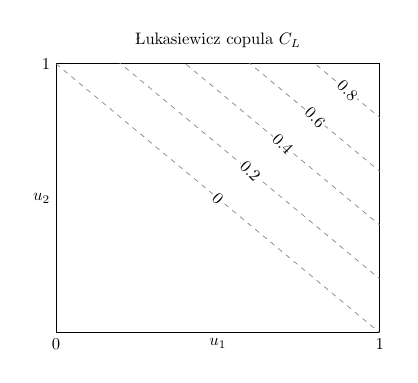
\begin{tikzpicture}[scale=0.6]
        \begin{axis}[
            xmin=0,xmax=1,
            ymin=0,ymax=1,
            xtick={0, 0.5, 1},
		    xticklabels={$0$, $u_1$, $1$},
		    ytick={0.5, 1},
		    yticklabels={$u_2$, $1$},
		    xtick style={draw=none},
		    ytick style={draw=none},
            title={\L ukasiewicz copula $C_L$},
            ]
            \addplot [domain=0:1,samples=40,style=dashed,color=gray]({x},{1-x});
            \addplot [domain=0:1,samples=40,style=dashed,color=gray]({x},{1.2-x}); 
            \addplot [domain=0:1,samples=40,style=dashed,color=gray]({x},{1.4-x}); 
            \addplot [domain=0:1,samples=40,style=dashed,color=gray]({x},{1.6-x}); 
            \addplot [domain=0:1,samples=40,style=dashed,color=gray]({x},{1.8-x});

            \node[rotate=-45, fill=white, rounded corners=2pt, inner sep=1pt] (x) at (0.5, 0.5) {0};
            \node[rotate=-45, fill=white, rounded corners=2pt, inner sep=1pt] (x) at (0.6, 0.6) {0.2};
            \node[rotate=-45, fill=white, rounded corners=2pt, inner sep=1pt] (x) at (0.7, 0.7) {0.4};
            \node[rotate=-45, fill=white, rounded corners=2pt, inner sep=1pt] (x) at (0.8, 0.8) {0.6};
            \node[rotate=-45, fill=white, rounded corners=2pt, inner sep=1pt] (x) at (0.9, 0.9) {0.8};
        \end{axis}
        \end{tikzpicture}\quad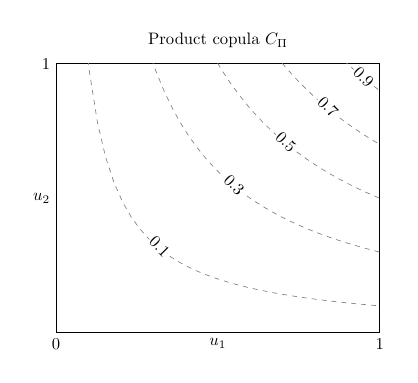
\begin{tikzpicture}[scale=0.6]
        \begin{axis}[
            xmin=0,xmax=1,
            ymin=0,ymax=1,
            xtick={0, 0.5, 1},
		    xticklabels={$0$, $u_1$, $1$},
		    ytick={0.5, 1},
		    yticklabels={$u_2$, $1$},
		    xtick style={draw=none},
		    ytick style={draw=none},
            title={Product copula $C_\Pi$},
            ]
            \addplot[domain=0:1,samples=40,style=dashed,color=gray]({x},{0.1/x});
            \addplot[domain=0:1,samples=40,style=dashed,color=gray]({x},{0.3/x}); 
            \addplot[domain=0:1,samples=40,style=dashed,color=gray]({x},{0.5/x}); 
            \addplot[domain=0:1,samples=40,style=dashed,color=gray]({x},{0.7/x}); 
            \addplot[domain=0:1,samples=40,style=dashed,color=gray]({x},{0.9/x});

            \node[rotate=-45, fill=white, rounded corners=2pt, inner sep=1pt] (x) at (0.32, 0.32) {0.1};
            \node[rotate=-45, fill=white, rounded corners=2pt, inner sep=1pt] (x) at (0.55, 0.55) {0.3};
            \node[rotate=-45, fill=white, rounded corners=2pt, inner sep=1pt] (x) at (0.71, 0.71) {0.5};
            \node[rotate=-45, fill=white, rounded corners=2pt, inner sep=1pt] (x) at (0.84, 0.84) {0.7};
            \node[rotate=-45, fill=white, rounded corners=2pt, inner sep=1pt] (x) at (0.95, 0.95) {0.9};
            
        \end{axis}
        \end{tikzpicture}\quad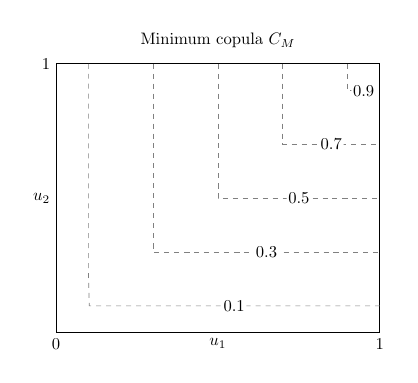
\begin{tikzpicture}[scale=0.6]
        \begin{axis}[
            xmin=0,xmax=1,
            ymin=0,ymax=1,
            xtick={0, 0.5, 1},
		    xticklabels={$0$, $u_1$, $1$},
		    ytick={0.5, 1},
		    yticklabels={$u_2$, $1$},
		    xtick style={draw=none},
		    ytick style={draw=none},
            title={Minimum copula $C_M$},
            ]
            \addplot [domain=0:1,samples=40,style=dashed,color=gray]({max(x, 0.1)},{max(1-x/0.1,0.1)});
            \addplot [domain=0:1,samples=40,style=dashed,color=gray]({max(x, 0.3)},{max(1-x/0.3,0.3)});
            \addplot [domain=0:1,samples=40,style=dashed,color=gray]({max(x, 0.5)},{max(1-x/0.5,0.5)});
            \addplot [domain=0:1,samples=40,style=dashed,color=gray]({max(x, 0.7)},{max(1-x/0.7,0.7)});
            \addplot [domain=0:1,samples=40,style=dashed,color=gray]({max(x, 0.9)},{max(1-x/0.9,0.9)});

            \node[fill=white, rounded corners=2pt, inner sep=1pt] (x) at (0.55, 0.1) {0.1};
            \node[fill=white, rounded corners=2pt, inner sep=1pt] (x) at (0.65, 0.3) {0.3};
            \node[fill=white, rounded corners=2pt, inner sep=1pt] (x) at (0.75, 0.5) {0.5};
            \node[fill=white, rounded corners=2pt, inner sep=1pt] (x) at (0.85, 0.7) {0.7};
            \node[fill=white, rounded corners=2pt, inner sep=1pt] (x) at (0.95, 0.9) {0.9};
        \end{axis}
        \end{tikzpicture}
    \caption{Bird view of the \L ukasiewicz, product and Min copulas for $n=2$. Dashed gray lines represent isolines of the copulas.}
    \label{fig:copulas}
\end{figure}


{\renewcommand{\arraystretch}{2}%
\begin{table}[!ht]
    \centering
    \begin{tabular}{|c|c|c|c|c|}
        \hline
        Family & $C(u_1,u_2)$ & $\theta \in $ & D-convex & D-concave \\
        \hline\hline
        Ali-Mikhail-Haq & $\frac{u_1u_2}{1-\theta(1-u_1)(1-u_2)}$ & $[-1,1)$ & $\theta\leqslant0$ & $0\leqslant\theta$ \\
        \hline
        Clayton & $\left[\max(u_1^{-\theta}+u_2^{-\theta}-1,0)\right]^{-1/\theta}$ & $[-1,\infty)\backslash\{0\}$ & $\theta<0$ & $0<\theta$ \\
        \hline
        Frank & $-\frac{1}{\theta}\ln(1+\frac{(e^{-\theta u_1}-1)(e^{-\theta u_2}-1)}{e^{-\theta}-1})$ & $\mathbb{R}\backslash \{0\}$ & $\theta<0$ & $0<\theta$ \\
        \hline
        Gumbel & $u_1u_2\exp(-\theta \ln{u_1}\ln{u_2})$ & $(0,1]$ & $\theta\in(0,1]$  & Never \\
        \hline
    \end{tabular}
    \caption{Examples of families of copulas in the case $n=2$ which can be generated using a parameter \( \theta \). D-convexity/concavity is detailed in section \ref{sec:dconvexity}}
    \label{tab:familiy_of_copula}
\end{table}}\commanue{alors la notation $0\leqslant\theta$ c'est pas la plus lisible disons qu'on a plutôt tendance à mettre $\theta\geqslant 0$ }

\begin{remark}
	As a copula is also a multivariate CDF, one can imagine an ``imprecise'' copula similarly to what can be done with univariate probability distribution (see section \ref{sec:imprecise_probabilities}). Imprecise copula allow to model partially known dependencies, but can be hard to manipulate at times, as for instance the lower and upper bounds of an imprecise copula are not necessarily copulas themselves. In this thesis, we will not consider imprecise copulas.
\end{remark}

\subsection{Directional convexity/concavity for copulas}\label{sec:dconvexity}
This section will investigate a property shared by some copulas called directional convexity/concavity. This is more of a theoretical contribution, as we do not exploit them in the applications to stereo-photogrammetry in chapters \ref{chap:propagating} and \ref{chap:epistemic_uncertainty}. However, we will see that those properties are shared by many common families of copulas. We also use them to prove a specific relationship between multivariate uncertainty models in sections \ref{subsec:pboxes} and \ref{subsec:multiple_models}. For readers that do not want to dive into details regarding directional convexity/concavity, we advise to consider only definition \ref{def:convex} and the main result of this section which is presented in equation \eqref{eq:convex_diff_hvol}.

\begin{definition}[D-convexity, D-concavity]\label{def:convex}
    A copula $C$ is called directionally convex (D-convex) \cite{alvoni_dierent_2007} if for every $(u_1,\dots,u_n)\in[0,1]^n$, $(v_1, \dots, v_n)\in[0,1]^n$, $i\in\opi1,n\cli$ and $t\in[0,1]$ it verifies:
    \begin{align}
        C(u_1,\dots, tu_i+(1-t)v_i,\dots, u_n) ~\leqslant~&t\cdot C(u_1,\dots, u_i,\dots, u_n)\nonumber\\
        &+ (1-t)\cdot C(u_1,\dots, v_i,\dots, u_n)\label{eq:convex_copula}
    \end{align}
    In other words, the copula is convex when fixing all but one of its variables. A copula is called directionally concave (D-concave) if the inequality is reversed.
\end{definition}

\begin{remark}
    D-convexity/D-concavity is quite common in known families of copulas. The following paragraphs details this property for copulas presented in table \ref{tab:familiy_of_copula}, in the case $n=2$.
    As the copulas presented are symmetric regarding their variables, D-convexity/D-concavity is only detailed for $u_1$. We assume that \( \theta \) always belong to the domain of definition detailed in table \ref{tab:familiy_of_copula}, and that \(u_1, u_2\) are in \([0, 1]\). Finally, for the Clayton and Gumbel family, the copula is defined by continuous extension in cases $u_1=0$ and $u_2=0$. 
    \begin{description}
        \item[Ali-Mikhail-Haq copula] This copula is two times differentiable, and its second order partial derivative is
        $$\frac{\partial^2 C}{\partial {u_1}^2}=u_2(1-\theta(1-u_2))\frac{-2\theta(1-u_2)}{(1-\theta(1-u_1)(1-u_2))^3}$$
        Thus the Ali-Mikhail-Haq copula is D-convex for $\theta\in[-1,0]$ and D-concave for $\theta\in[0,1)$.\commanue{Peut-être ajouter quelque part, la copule est convexe si et seulement si sa dérivée seconde est à valeurs positives ou nulles. }
        \item[Clayton copula] This copula is not always differentiable on all of its domain, depending on the value retained in the maximum function. It is however continuous as it is the maximum of two continuous function. For convenience, we work with $(u_1, u_2)$ in $\mathbb{I}^2$, where $\mathbb{I}$ is the open unit interval (the closed unit interval is then covered by continuity). Let $u_2\in\mathbb{I}$. We split the possible range $\mathbb{I}$ of $u_1$ in two:
    \begin{itemize}
        \item the first domain $\mathcal{D}_1^{\theta,u_2}$ is where $u_1^{-\theta}+u_2^{-\theta}-1\leqslant0$, and thus $C(u_1, u_2)=0$. Here, $\frac{\partial^2 C}{\partial {u_1}^2}=0$ and the copula is both D-convex and D-concave.
        \item the second domain $\mathcal{D}_2^{\theta,u_2}$ is where $u_1^{-\theta}+u_2^{-\theta}-1>0$ and thus $C(u_1, u_2)\geqslant0$. Here it holds that
        $$\frac{\partial^2 C}{\partial {u_1}^2}=(1+\theta)(1-u_2^{-\theta})u_1^{-2-\theta}(u_1^{-\theta}+u_2^{-\theta}-1)^{-2-\frac{1}{\theta}}$$
        Because of the definition of $\mathcal{D}_2^{\theta,u_2}$, the sign of $\frac{\partial^2 C}{\partial {u_1}^2}$ on $\mathcal{D}_2^{\theta,u_2}$ is that of $1-u_2^{-\theta}$.
    \end{itemize}
    
    If $\theta>0$, then $D^\theta_2=\mathbb{I}$ and $\frac{\partial^2 C}{\partial {u_1}^2}\leqslant0$ which means that the copula is D-concave on all of its domain.
    
    The case where $\theta<0$ is less straightforward. In that case, $\frac{\partial^2 C}{\partial {u_1}^2}\geqslant0$ on $\mathcal{D}_2^{\theta,u_2}$. The restrictions of the copula to $\mathcal{D}_1^{\theta,u_2}$ and $\mathcal{D}_2^{\theta,u_2}$ are both D-convex, but we need to prove that it is still true on their union. Let $u_1\in\mathcal{D}_1^{\theta,u_2}$, $v_1\in\mathcal{D}_2^{\theta,u_2}$ and $t\in[0,1]$. We note $w_1=(1-u_2^{-\theta})^{-\frac{1}{\theta}}$, such that $\mathcal{D}_1^{\theta,u_2}=]0,w_1]$ and $\mathcal{D}_2^{\theta,u_2}=]w_1, 1[$. By continuity, $C$ is D-convex on $\mathcal{D}_2^{\theta,u_2}\bigcup\{w_1\}$. Because $u_1,w_1\in \mathcal{D}_1^{\theta,u_2}$, it holds that:
        \begin{eqnarray*}
            tC(u_1,~u_2)+(1-t)C(v_1,~u_2) &=& tC(w_1,~u_2)+(1-t)C(v_1,~u_2)\\
            &\geqslant& C(tw_1+(1-t)v_1,~u_2)\\
            &&\text{by convexity of $C$ on $\mathcal{D}_2^{\theta,u_2}\bigcup\{w_1\}$}\\
            &\geqslant& C(tu_1+(1-t)v_1,~u_2)\\
            && \text{because $C$ is component-wise increasing}
        \end{eqnarray*}
    which, by definition \ref{def:convex}, proves that $C$ is D-convex on $\mathcal{D}_1^{\theta,u_2}\bigcup \mathcal{D}_2^{\theta,u_2}$. By continuity, $C$ is D-convex on all of its domain.
    \item[Frank copula] This copula is two times differentiable, and its second order partial derivative is
    $$\frac{\partial^2 C}{\partial {u_1}^2}=\frac{(e^{-\theta u_2}-1)e^{-\theta u_1}\theta(e^{-\theta u_2}-e^{-\theta} )}{(e^{-\theta}-1+(e^{-\theta u_1}-1)(e^{-\theta u_2}-1))^2}$$
    If $\theta\geqslant0$ then $\frac{\partial^2 C}{\partial {u_1}^2}\leqslant 0$ and $C$ is D-concave. If $\theta\leqslant0$ then $\frac{\partial^2 C}{\partial {u_1}^2}\geqslant 0$ and $C$ is D-convex.
    \item[Gumbel copula] This copula is two times differentiable on $]0,1]^2$, and its second order partial derivative is
    $$\frac{\partial^2 C}{\partial {u_1}^2}=-\theta\frac{u_2}{u_1}\ln(u_2)(1-\theta\ln(u_2))e^{-\theta\ln(u_1)\ln(u_2)}$$
    It holds that for all $\theta\in(0,1]$, $\frac{\partial^2 C}{\partial {u_1}^2}\geqslant0$. By continuity, $C$ is always D-convex.
    \end{description}
    
    As there is no explicit formula for the family of multivariate Gaussian copulas, it is difficult to prove its D-concavity or D-convexity. However, numerical approximations in the case $n=2$ seem to indicate that a Gaussian copula would be D-convex if its marginals are positively correlated, and D-concave if they are negatively correlated. Figure \ref{fig:gaussian_copula_simu} present those observations, with solid lines representing positive correlation, and dashed lines representing negative correlations. In the case $n>2$, the copula can be neither D-convex nor D-concave depending on the value of the correlation matrix. An example of this statement is provided in figure \ref{fig:gaussian_copula_simu_n3}.
\end{remark}

\begin{figure}
    \centering
    \begin{subfigure}{0.4\linewidth}
        \centering
        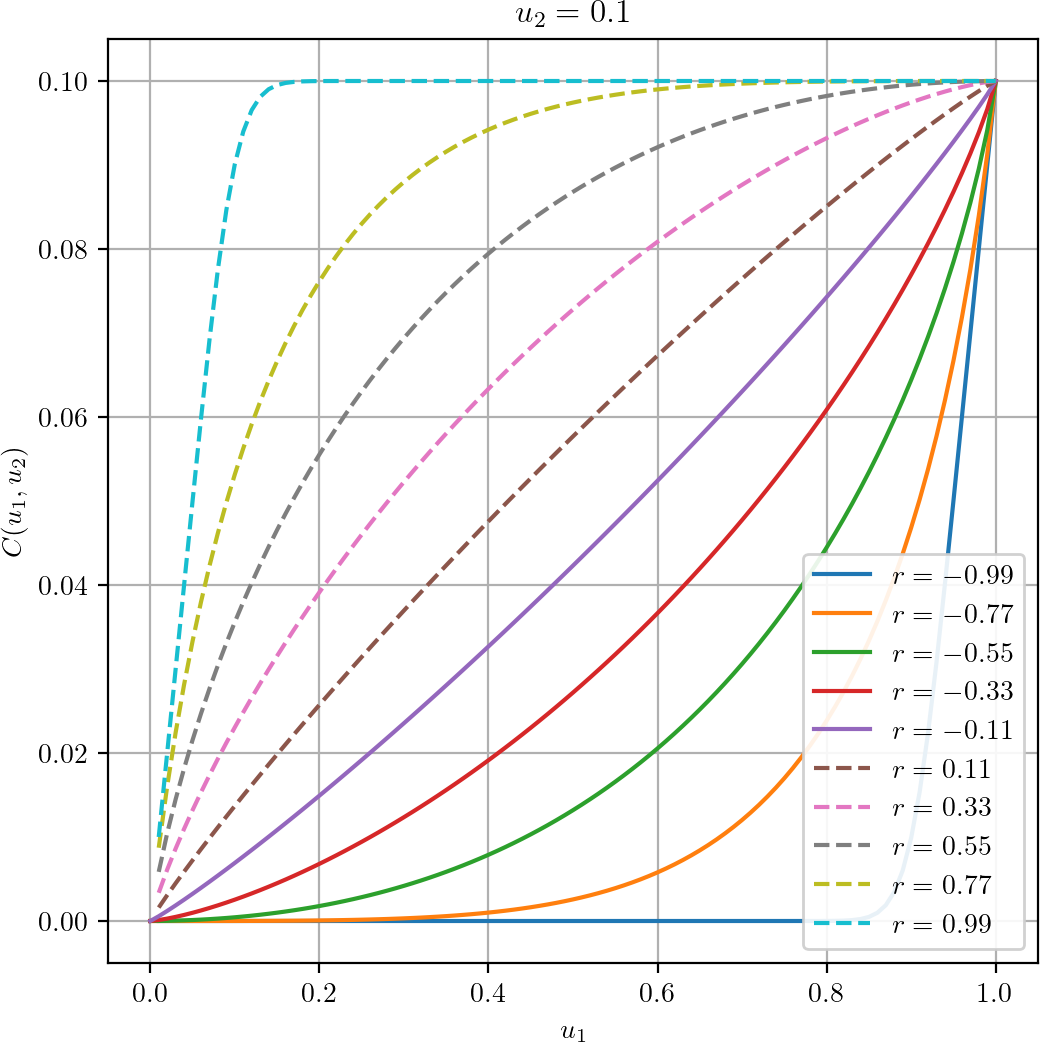
\includegraphics[width=\linewidth]{Images/Chap_2/Gaussian_copula/gaussian_copula_0.png}
    \end{subfigure}\hfill
    \begin{subfigure}{0.4\linewidth}
        \centering
        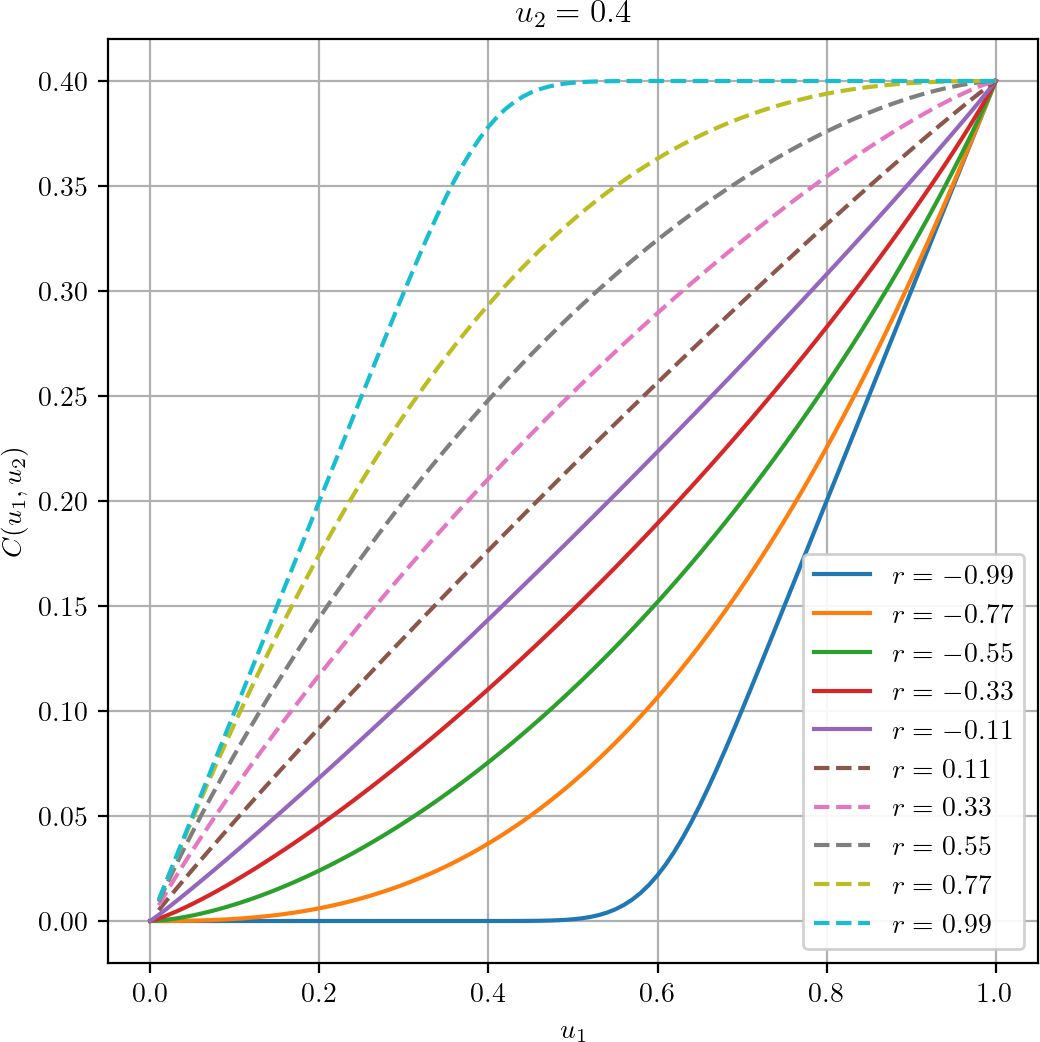
\includegraphics[width=\linewidth]{Images/Chap_2/Gaussian_copula/gaussian_copula_1.png}
    \end{subfigure}\hfill
    \begin{subfigure}{0.4\linewidth}
        \centering
        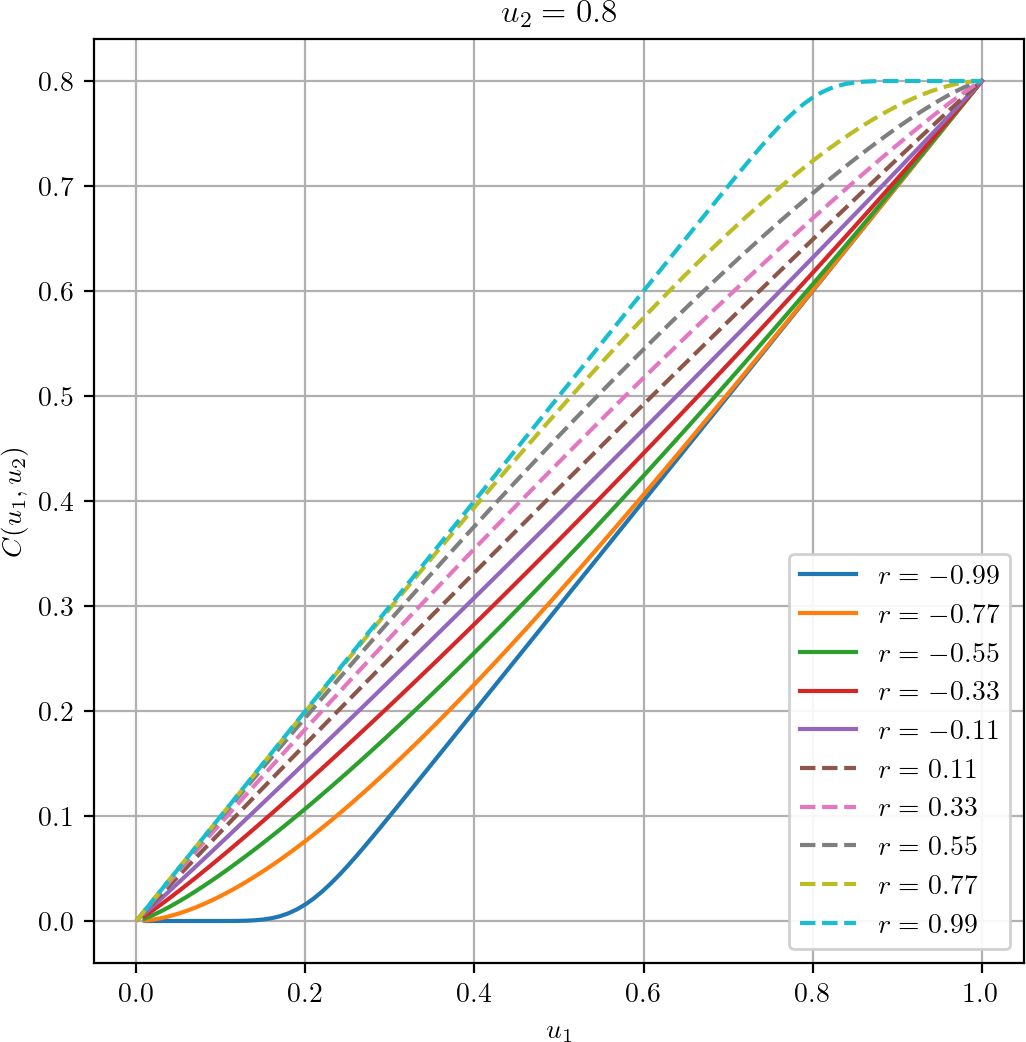
\includegraphics[width=\linewidth]{Images/Chap_2/Gaussian_copula/gaussian_copula_2.png}
    \end{subfigure}
    \caption{Gaussian 2-copulas in the direction $u_1$ for different $u_2$. Each figure present different plots for correlations $r$ between $u_1$ and $u_2$ ranging in $[-1,1]$. Solid lines represent negative correlation, while dashed lines represent positive correlations.}
    \label{fig:gaussian_copula_simu}
\end{figure}

The rest of this section will present different results regarding D-convex and D-concave copulas, leading to the main result of this section presented in proposition \ref{prop:convex_diff_hvol}.

\begin{figure}
    \centering
    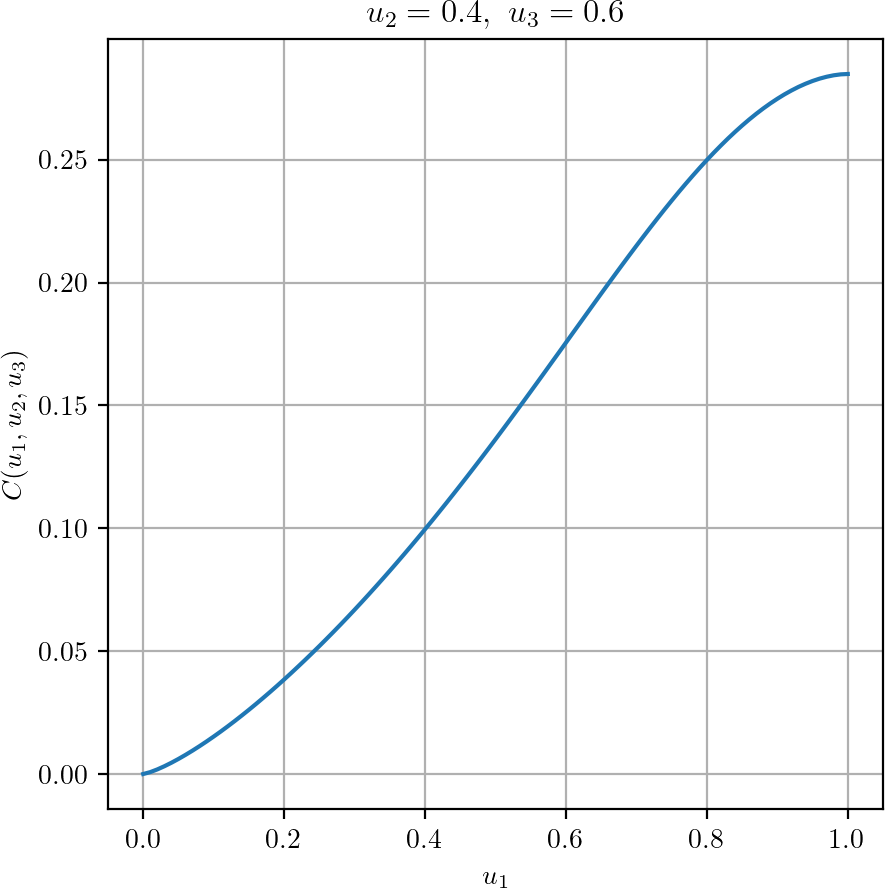
\includegraphics[width=0.5\linewidth]{Images/Chap_2/Gaussian_copula/gaussian_copula_n3.png}
    \caption{Directional cut of a Gaussian 3-copula with in the direction $u_1$, with $R=\begin{bmatrix} 1 & -0.4 & 0.7\\ -0.4 & 1 & 0.3\\ 0.7 & 0.3 & 1 \end{bmatrix}$, $u_2=0.4$ and $u_3=0.6$. The copula is neither D-convex nor D-concave}
    \label{fig:gaussian_copula_simu_n3}
\end{figure}

\begin{remark}
    All D-convex copulas $C$ are dominated by the product copula. Similarly, all D-concave copulas dominate the product copula.

    Consider a D-convex copula $C$, and let $(u_1, \dots, u_n)\in[0,1]^n$.
    \begin{eqnarray*}
        C(u_1,\dots, u_n) &=& C((1-u_1)\cdot0+u_1\cdot 1, u_2, \dots, u_n)\\
        &\leqslant& (1-u_1)C(0, u_2,\dots, u_n)+u_1C(1, u_2, \dots, u_n)\\
        &=& u_1C(1, u_2,\dots, u_n)\commanue{alors moi je laisserais le symbole $\leqslant$ et pas $=$}
    \end{eqnarray*}
    Doing the same for $u_2,\dots,u_n$ yields:
    \begin{eqnarray*}
        C(u_1,\dots, u_n) &\leqslant& u_1\dots u_nC(1,\dots,1) = u_1\dots u_n = C_\Pi(u_1,\dots,u_n)
    \end{eqnarray*}
    The proof for D-convexity is similar.
\end{remark}

\begin{proposition}\label{prop:sup_additivity}
    If $C$ is a D-convex copula, then it verifies for all $(u_1,\dots,u_n)\in[0,1]^n$, $(v_1,\dots,v_n)\in[0,1]^n$ \st $\forall i\in\opi1,n\cli$, $u_i+v_i\leqslant 1$:
    \begin{eqnarray}
        C(u_1,\dots,u_i+v_i,\dots,u_n)\geqslant& &C(u_1,\dots,u_i,\dots,u_n)\nonumber\\
        &+ &C(u_1,\dots,v_i,\dots,u_n)\label{eq:convex_sum}
    \end{eqnarray}
    Similarly, if $\forall i\in\opi1,n\cli$, $u_i-v_i\geqslant 0$, it verifies:
    \begin{eqnarray}
        C(u_1,\dots,u_i-v_i,\dots,u_n)\leqslant& &C(u_1,\dots,u_i,\dots,u_n)\nonumber\\
        &- &C(u_1,\dots,v_i,\dots,u_n)\label{eq:convex_diff}
    \end{eqnarray}
    The inequalities are reversed for D-concave copulas.
\end{proposition}

\begin{proof}
    Let $(u_1,\dots,u_n)\in[0,1]^n$, $(v_1,\dots,v_n)\in[0,1]^n$ \st $\forall i\in\opi1,n\cli$, $u_i+v_i\leqslant 1$. Let $i\in\opi1,n\cli$. Applying the definition of convexity \eqref{eq:convex_copula} with $v_i=0$ yields:
    \begin{eqnarray*}
        \forall t\in[0,1],~C(u_1,\dots,tu_i,\dots, u_n) \leqslant tC(u_1,\dots, u_n)
    \end{eqnarray*}
    
    Let $w_i=u_i+v_i\in ]0,1]$ (the case where $u_i=0$ or $v_i=0$ is trivial). It is possible to write $u_i=tw_i$ and $v_i=(1-t)w_i$, with $t=\frac{u_i}{w_i}\in[0,1]$. Then it holds that:
    \begin{eqnarray*}
            C(u_1,\dots,u_i,\dots,u_n) =& C(u_1, \dots, tw_i,\dots, u_n) &\leqslant tC(u_1, \dots, w_i, \dots, u_n)\\
            C(u_1,\dots,v_i,\dots,u_n) =& C(u_1, \dots, (1-t)w_i,\dots, u_n) &\leqslant (1-t)C(u_1, \dots, w_i, \dots, u_n)
    \end{eqnarray*}
    Summing the above equations yields:
    \begin{eqnarray*}
        C(u_1,\dots,u_i,\dots,u_n) + C(u_1,\dots,v_i,\dots,u_n) &\leqslant& C(u_1, \dots, w_i, \dots, u_n)\\
        &\leqslant& C(u_1, \dots, u_i+v_i, \dots, u_n)
    \end{eqnarray*}
    which proves equation \eqref{eq:convex_sum}.

    Let $w_i=u_i-v_i\in [0,1]$, clearly $w_i+v_i\leqslant1$. Using equation \eqref{eq:convex_sum}, it holds that:
    \begin{align*}
        &C(u_1,\dots,w_i,\dots,u_n) + C(u_1,\dots,v_i,\dots,u_n) &\leqslant~&C(u_1, \dots, w_i+v_i, \dots, u_n)\\
        \Leftrightarrow~ &C(u_1,\dots,w_i,\dots,u_n) &\leqslant~&C(u_1, \dots, w_i+v_i, \dots, u_n)\\
        &&&-C(u_1,\dots,v_i,\dots,u_n)\\
        \Leftrightarrow~ &C(u_1,\dots,u_i-v_i,\dots,u_n) &\leqslant~&C(u_1, \dots, u_i, \dots, u_n)\\
        &&&-C(u_1,\dots,v_i,\dots,u_n)
    \end{align*}
    which proves equation \eqref{eq:convex_diff}.
\end{proof} 

\begin{proposition}\label{prop:convex_diff_hvol}
    If $C$ is a D-convex copula, then it verifies for all $(u_1,\dots,u_n)\in[0,1]^n$, $(v_1,\dots,v_n)\in[0,1]^n$ \st $\forall i\in\opi1,n\cli$, $u_i-v_i\geqslant 0$:
    \begin{eqnarray}
        C(u_1-v_1,\dots,u_i-v_i,\dots,u_n-v_n)\leqslant& &H^{u_1,\dots,u_i,\dots,u_n}_{v_1,\dots,v_i,\dots,v_n}\label{eq:convex_diff_hvol}
    \end{eqnarray}
    where $H$ is the H-volume of $C$. The inequality is reversed for D-concave copulas.
\end{proposition}

\begin{proof}
    The result is straightforward by induction using equation \eqref{eq:convex_diff}.
\end{proof}

\subsection{Sampling from a Copula}\label{sec:sampling_copula}
As a copula represent the CDF of a multivariate random variable, it is possible to sample from it. This section details a method for sampling from copulas in general, and a special method for sampling from Gaussian copulas. For simplicity, let us first present a method for sampling in the case $n=2$. Given a copula $C$, and two CDF $F_X$ and $F_Y$, a method to generate a pair of observations $(x, y)$ from a joint CDF $C(F_X, F_Y)$ is the following:

\begin{itemize}
    \item Sample two independent samples $u_1, u_2$ from a uniform distribution on [0,1]
    \item Set $v=\partial C^{-1}(u_2)$ where $\partial C^{-1}$ is the quasi-inverse of the partial derivative of $C$ regarding its first variable (which exists almost everywhere and is invertible).
    \item We now have a sample $(u_1, v)$ from a multivariate random. Its marginals follow a uniform distribution on $[0,1]$, and its associated copula is $C$.
    \item The desired pair is $(x_1,x_2) = (F^{-1}_X(u_1), F^{-1}_Y(v))$, with $F_X^{-1}$, $F_Y^{-1}$ being the quasi-inverses of the marginals CDFs.
\end{itemize}

We do not present the $n$-dimensional general case here as it is a bit more complex, but it can be found in \cite{cherubini_copula_2004}. However, drawing samples from a Gaussian $n$-copula with a correlation matrix $R$ are simpler to obtain:
\begin{itemize}
    \item Compute the Cholesky decomposition $A$ of the correlation matrix $R$
    \item Draw $n$ independent random samples $u=(u_1, \dots, u_n)'$ from $\mathcal{N}(0,1)$, where $\mathcal{N}$ is the normal distribution.
    \item Set $v=Au$
    \item Set $w_k=\Phi(v_k)$ where $\Phi$ is the univariate normal cumulative distribution function
    \item The desired draw is $(x_1,\dots, x_n)=(F^{-1}_1(w_1), \dots, F^{-1}_n(w_n))$ with $F_i^{-1}$, being the quasi-inverse of the $i$-th marginal CDF.
\end{itemize}
\commanue{Alors il manque une conclusion un truc, là ça termine un peu de manière abrupte, transition donc ;)}
\pagebreak
\blankpage